\documentclass[]{article}
\usepackage{caption,subcaption,graphicx,float,url,amsmath,amssymb,tocloft}
\usepackage[hidelinks]{hyperref}
\usepackage[toc,acronym,nonumberlist]{glossaries}
\setacronymstyle{long-short}
\usepackage{glossaries-extra}
\graphicspath{{figs/}} 
\setlength{\cftsubsecindent}{0em}
\setlength{\cftsecnumwidth}{3em}
\setlength{\cftsubsecnumwidth}{3em}

%opening
\title{
	Notes from Origins of Life\\
	Week 3: Chemical Commonalities
}

\author{Simon Crase}

\makeglossaries

\loadglsentries{glossary-entries}

\renewcommand{\thesection}{3.\arabic{section}}
\renewcommand{\glstextformat}[1]{\textbf{\em #1}}

\begin{document}

\maketitle

\begin{abstract}
 	These are my notes from Week 3 of the \gls{gls:SFI} Origins of Life Course\cite{sfi2019}. The course aims to push the field of Origins of Life research forward by bringing new and synthetic thinking to the question of how life emerged from an abiotic world.\\
  	The content and images contained herein are the intellectual property of the Santa Fe Institute, with the exception of any errors in transcription, which are my own.
  	These notes are distributed in the hope that they will be useful,
  	but without any warranty, and without even the implied warranty of
  	merchantability or fitness for a particular purpose. All feedback is welcome,
  	but I don't necessarily undertake to do anything with it.
\end{abstract}

\setcounter{tocdepth}{2}
\tableofcontents

\listoffigures

\section{Introduction}

This week is a more detailed look at biochemistry: biological information encoded in chemistry; the chemical processes that drive organization; and how life extracts energy from its environment.

\section{DNA as Information}
Lecturer: Michael Lachmann, \gls{gls:SFI}

\subsection{DNA Modification}

\begin{figure}[H]
	\caption{The 4 Nucleotides in DNA}\label{fig:Nucleotides} 
	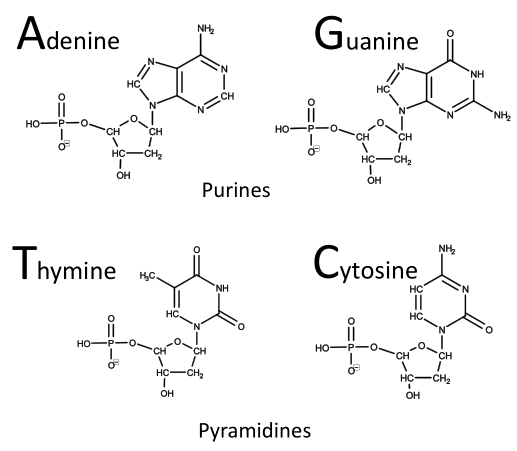
\includegraphics[width=0.9\textwidth]{Nucleotides}
\end{figure}

\begin{figure}[H]
	\caption{A closer look at one Nucleotide, Adenine}\label{fig:NucleotideAdenine} 
	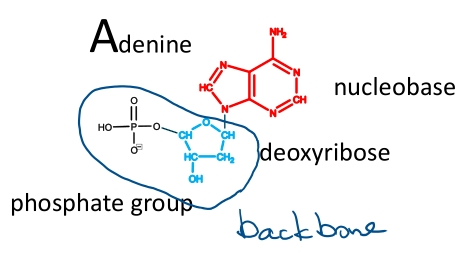
\includegraphics[width=0.9\textwidth]{NucleotideAdenine}
\end{figure}

Figure \ref{fig:NucleotideDNARNA} shows the only chemical difference between DNA and RNA: the extra OH group in RNA, which makes the molecule more active. DNA is more stable.
\begin{figure}[H]
	\caption{The only chemical difference between DNA and RNA }\label{fig:NucleotideDNARNA} 
	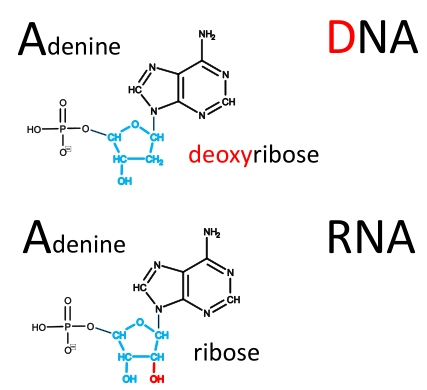
\includegraphics[width=0.9\textwidth]{NucleotideDNARNA}
\end{figure}

RNA uses Uracil instead of Thymine--Figure \ref{fig:NucleotideDNARNAThymineUracil}. Note that Thymine is Uracil with an extra methyl group, hence the alternative name $5-methyluracil$. The $5$ comes from the numbering of carbon atoms--see \ref{fig:NucleotidesCounting}
	
\begin{figure}[H]
	\caption{RNA uses Uracil instead of Thymine.} \label{fig:NucleotideDNARNAThymineUracil} 
	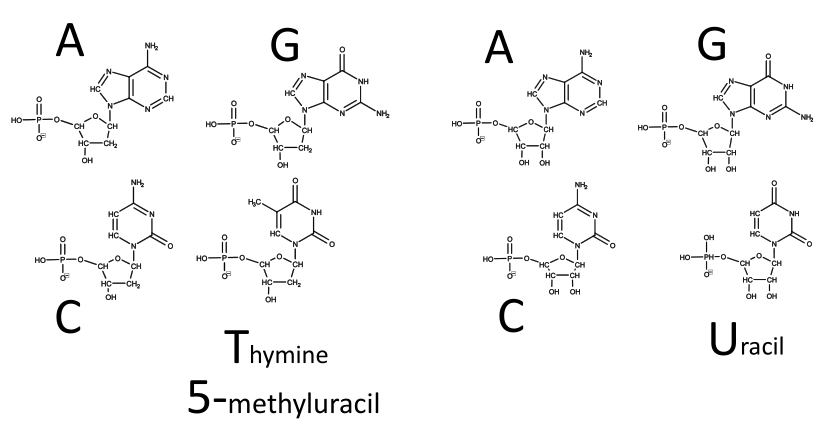
\includegraphics[width=0.9\textwidth]{NucleotideDNARNAThymineUracil}
\end{figure}

\begin{figure}[H]
	\caption{Numbering of carbon atoms in purines and pyrimidines. }\label{fig:NucleotidesCounting} 
	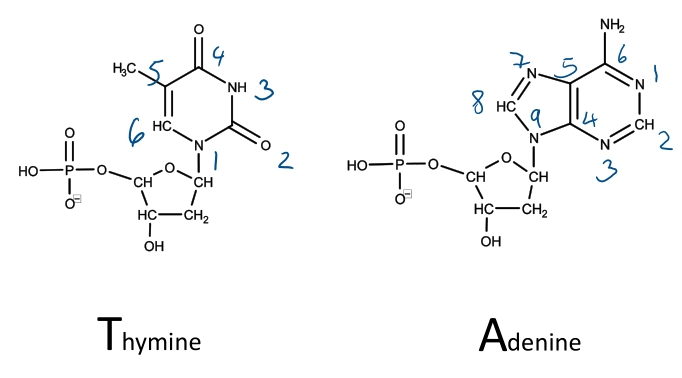
\includegraphics[width=0.9\textwidth]{NucleotidesCounting}
\end{figure}

\begin{figure}[H]
	\caption{A selection of 12 modified bases}\label{fig:ModifiedBases} 
	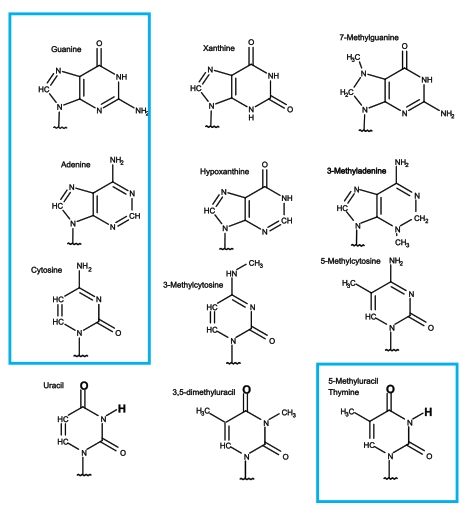
\includegraphics[width=0.9\textwidth]{ModifiedBases}
\end{figure}

\gls{gls:deamination}

Fugre \ref{fig:ModifiedDNA_Nucleobases} shows the 44 Modified DNA nucleobases that have actually been observed.\cite{sood2019dnamod},\cite{sood2019dnamod_website}

\begin{figure}[H]
	\caption{Modified DNA nucleobases } \label{fig:ModifiedDNA_Nucleobases} 
	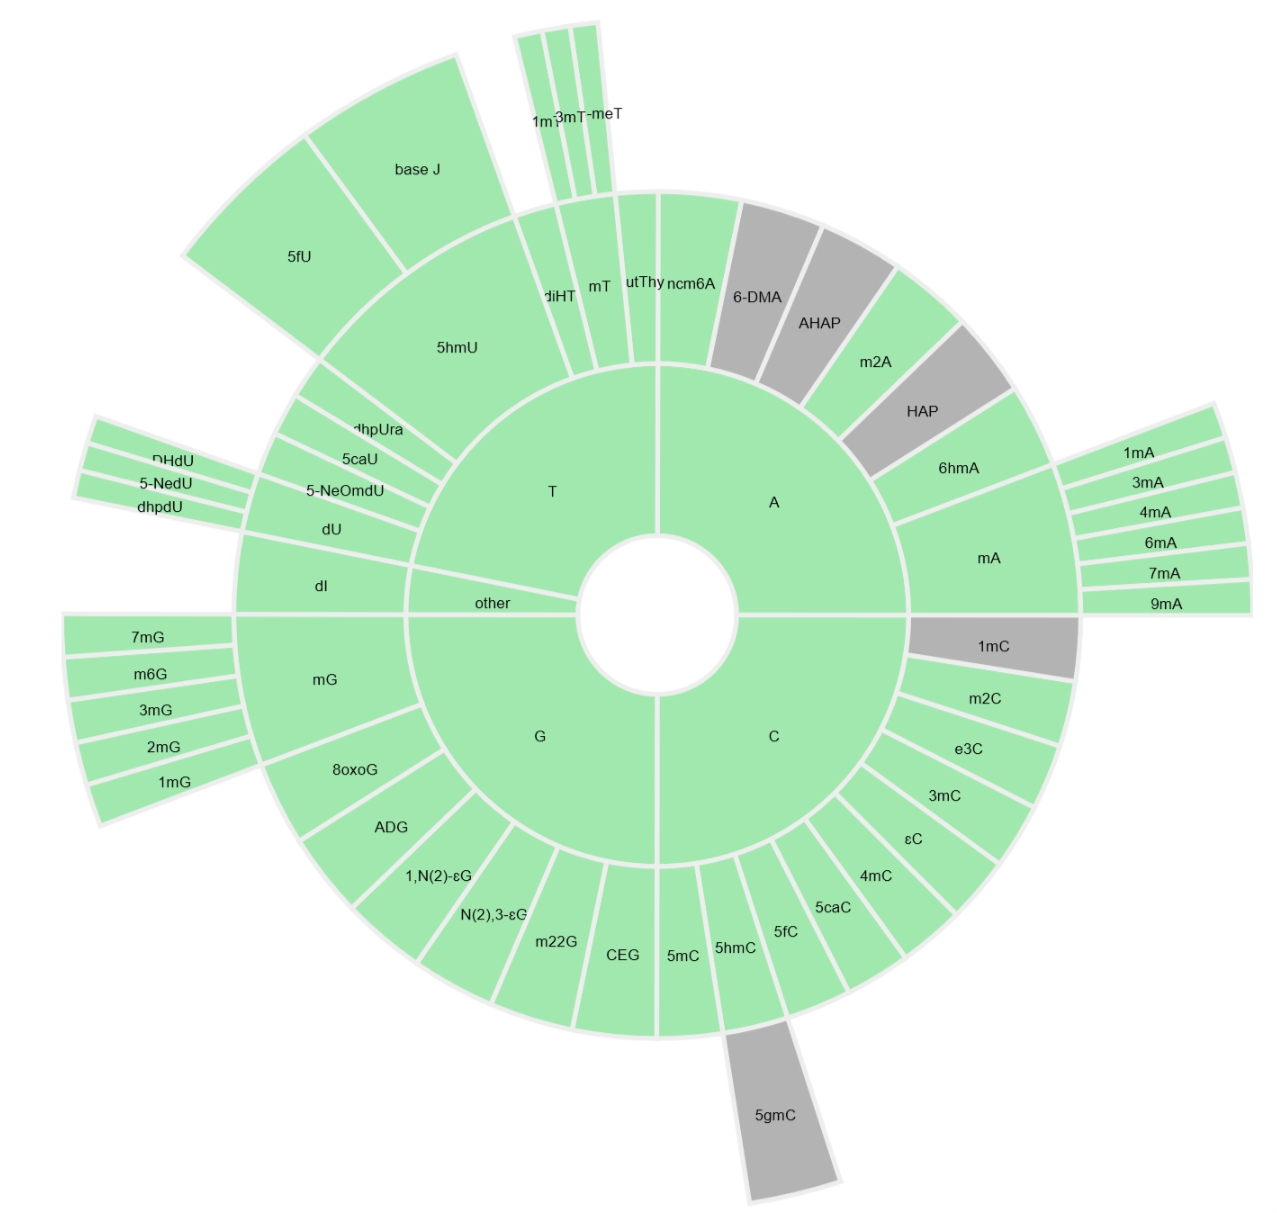
\includegraphics[width=0.9\textwidth]{ModifiedDNA_Nucleobases}
\end{figure}

The are a couple of bacteriophages, PBS1 and PBS2, that contain Uracil instead of thymine in their DNA\cite{hemphill1975bacteriophages}. Either the thymine has been replaced, or these phages are more primitive, and never used thymine.

When people talk about methylation of DNA, they usually mean $5-methylcytosine$, Figure \ref{fig:5methylcytosine}, even though there are many other ways to do it
\begin{figure}[H]
	\caption{$5-methylcytosine$ } \label{fig:5methylcytosine} 
	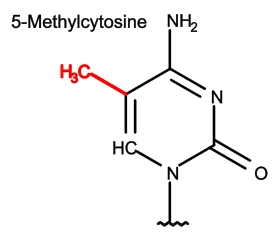
\includegraphics[width=0.9\textwidth]{5-methylcytosine}
\end{figure}

Methylation tends to occur when C is followed by G. The methylated versions are replicated us unmethylated C, but there is an enzyme, \gls{gls:DNAmethyltransferase}, which performs methylation, as shown in Figure \ref{fig:5-methylcytosine-in-action}. This can carry epigenetic changes across cell divisions, and sometimes across generations. This is important as it means that a lever cell can "remember" that is comes from a liver cell.
\begin{figure}[H]
	\caption{Methylation tends to occur when C is followed by G } \label{fig:5-methylcytosine-in-action} 
	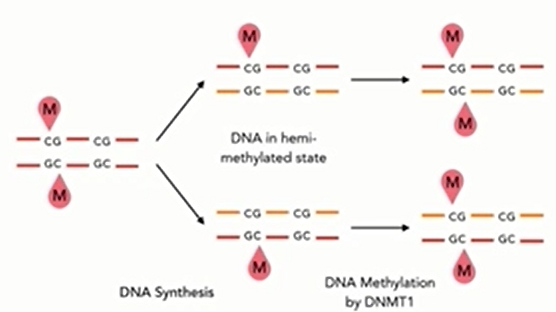
\includegraphics[width=0.9\textwidth]{5-methylcytosine-in-action}
\end{figure}

6-Methyladenine is also important--Figure \ref{fig:6-Methyladenine}-- in bacteria, where it carries information regarding the old strand versus the new. The methylation isn't very fast, so it can distinguish old from new. Section \ref{section:DNAasInfo2} shows how this is useful for repair.

\begin{figure}[H]
	\caption{6-Methyladenine is also important (palindromic sequence)} \label{fig:6-Methyladenine} 
	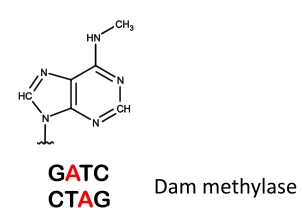
\includegraphics[width=0.9\textwidth]{6-Methyladenine}
\end{figure}

The values in Figure \ref{fig:ModifiedRNAdatabase} have been taken from the Modified RNA database \cite{agriss2019RNA}.

\begin{figure}[H]
	\caption{Modified RNA database} \label{fig:ModifiedRNAdatabase} 
	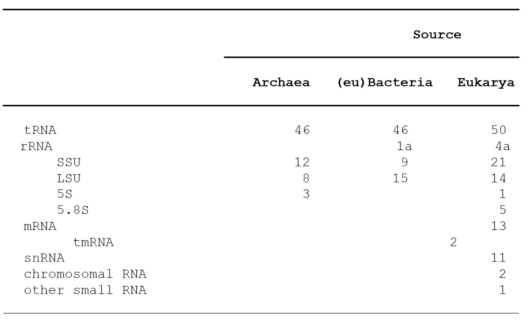
\includegraphics[width=0.9\textwidth]{ModifiedRNAdatabase}
\end{figure}

\textbf{Summary}

\begin{itemize}
	\item There are 44 known DNA modifications
	\item There are 112 known RNA modifications
	\item Many DNA modifications survive replication
	\item Some are replicated themselves
	\item Some modifications are functional:\begin{itemize}
		\item 5-methylcytosine (5mC)
		\item N6-methadenine (6mA)
		\item 5-hydroxymethylcytosine (5hmC)
		\item Some functional in RNA
		\item It is likely there are more, since this is a fairly new field.
	\end{itemize}
	\item How are they generated?
	\begin{itemize}
		\item Enzyme activity
		\item Damage
		\item Misincorporation
	\end{itemize}
\end{itemize}

Where did the modifications come from? They could be fairly new, and we use them in various ways; or maybe they tell us something about the origin of DNA. Maybe there are many enzymes left over from before we had sophisticated machinery for DNA replication.

\subsection{DNA base pairing}\label{section:DNAasInfo2}

Sarah added (forum):\begin{quote}
	The idea of Information part2 is that the thermodynamics alone cannot explain our high fidelity replication, and that our system of replicating DNA uses several compounding mechanisms to generate robust replication. While the first organisms likely lacked this process as the machinery to do this is very sophisticated, it is interesting to consider how early organisms would have survived with less controlled replication. Perhaps indicating that early organisms relied on gene products that had lower specificity?
\end{quote}

What generates and maintains the pairing rules?  How does DNA keep Error rate down to  $10^{-10}$ errors per (replication*base pair)?

Different pairing proceed at different rates--Figures \ref{fig:RightWrong} and \ref{fig:BindingDifference}, but this won't explain error rate of $10^{-10}$. At best it gives a factor of 60.
\begin{figure}[H]
	\caption{Different pairing proceed at different rates} \label{fig:RightWrong} 
	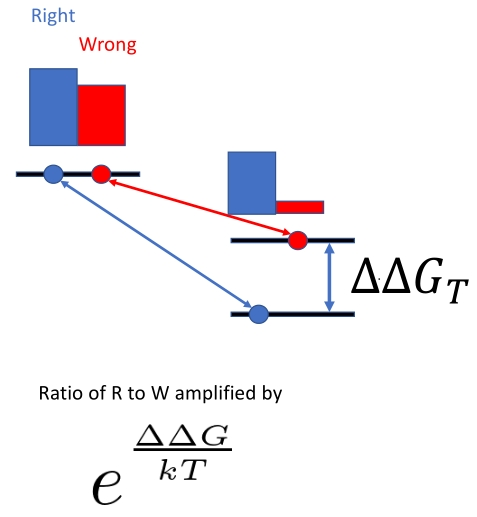
\includegraphics[width=0.9\textwidth]{RightWrong}
\end{figure}

\begin{figure}[H]
	\caption{Difference in Binding Energies for different pairings} \label{fig:BindingDifference} 
	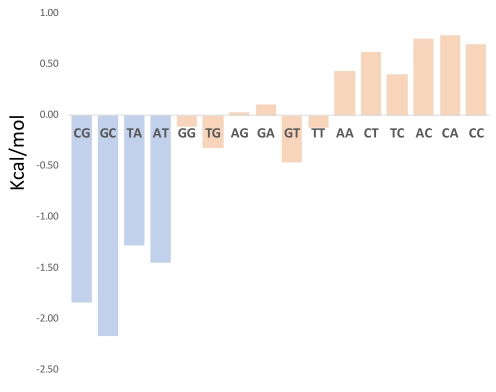
\includegraphics[width=0.9\textwidth]{BindingDifference}
\end{figure}
 Kinetic proofreading?
 
 
\textbf{Bases encountered by DNA polymerase}
	
\begin{itemize}
	\item Watson Crick pairs (CATG)
	\begin{itemize}
		\item  Only ~50 fold enrichment from pairing
		\item  Right base at 3-fold disadvantage
		\item  4 shapes valid
	\end{itemize}
	\item  “Valid” W-C extra bases (C*,6mA)
	\begin{itemize}
		\item Additional shapes valid
	\end{itemize}
	\item NTP from RNA
	\begin{itemize}
		\item Frequent
		\item Shape recognition
	\end{itemize}
	\item “Nonstandard” bases
	\begin{itemize}
		\item Rare, probably shape recognition
	\end{itemize}
\end{itemize}


Summary – it isn’t in the bases
\begin{itemize}
	\item Many bases exist in DNA/RNA
	\begin{itemize}
		\item Damage, modification, insertion
	\end{itemize}
	\item dNTP concentration is controlled
	\item DNA polymerase controls	pairing
	\item Large number of specific/general repair enzymes
\end{itemize}
\cite{kunkel2004dna}

\section{Water as a Driving Force for Organization}

Lecturer: Sarah Maurer

\begin{figure}[H]
	\caption{Chemical Energetics} \label{fig:ChemicalEnergetics} 
	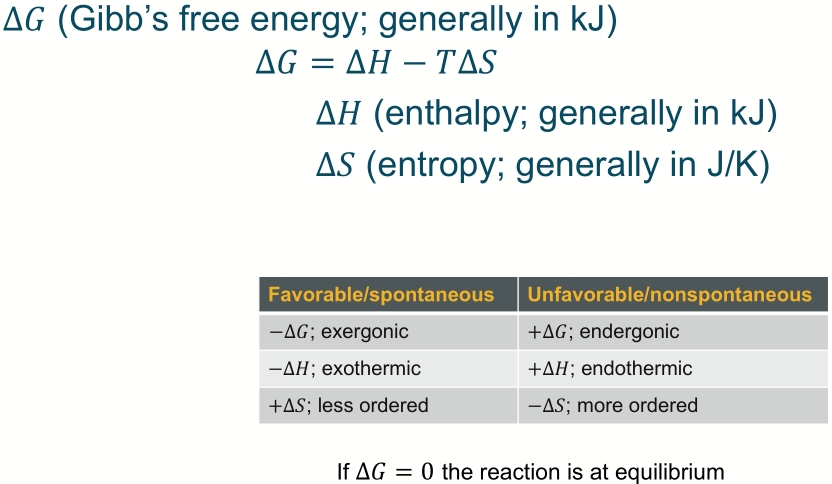
\includegraphics[width=0.9\textwidth]{ChemicalEnergetics}
\end{figure}

\begin{itemize}
	\item  Enthalpy is ”heat” energy, generally stored in bonds
	\begin{itemize}
		\item Breaking bonds takes enthalpy
		\item Making bonds releases enthalpy
	\end{itemize}
	\item Entropy is a measure of the number of occupied states of a system relative to the number of possible	states--Figure \ref{fig:EntropySugar}.
\end{itemize}

\begin{figure}[H]
	\caption{Entropy--$\frac{occupied}{total}$} \label{fig:EntropySugar} 
	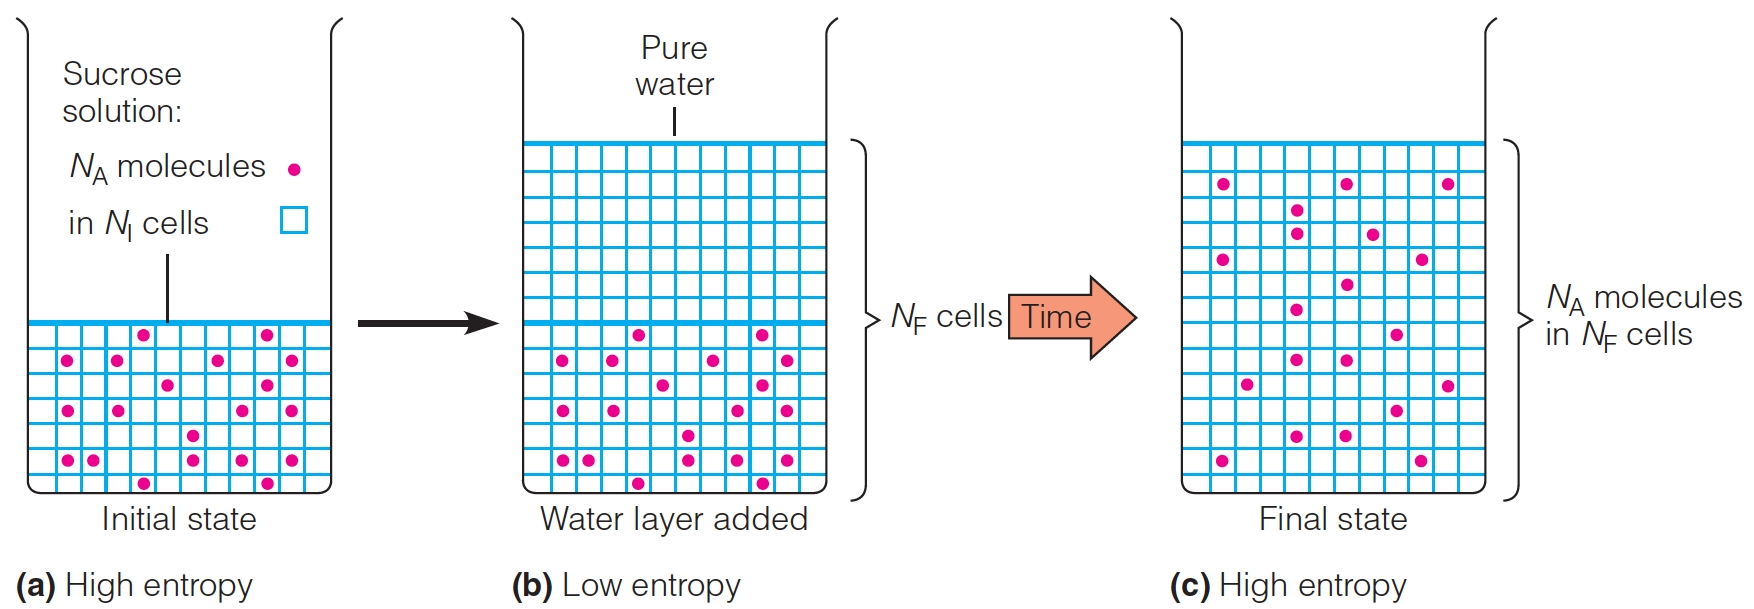
\includegraphics[width=0.9\textwidth]{EntropySugar}
\end{figure}

Very polar bonds can form hydrogen bonds (H-bonds): only F-H, N-H, or O-H, with
N, F or O.

\begin{figure}[H]
	\centering
		\caption{Very polar bonds can form hydrogen bonds} \label{fig:EnthalpyHydrogenBonds} 
	\begin{subfigure}{.5\textwidth}
		\centering
		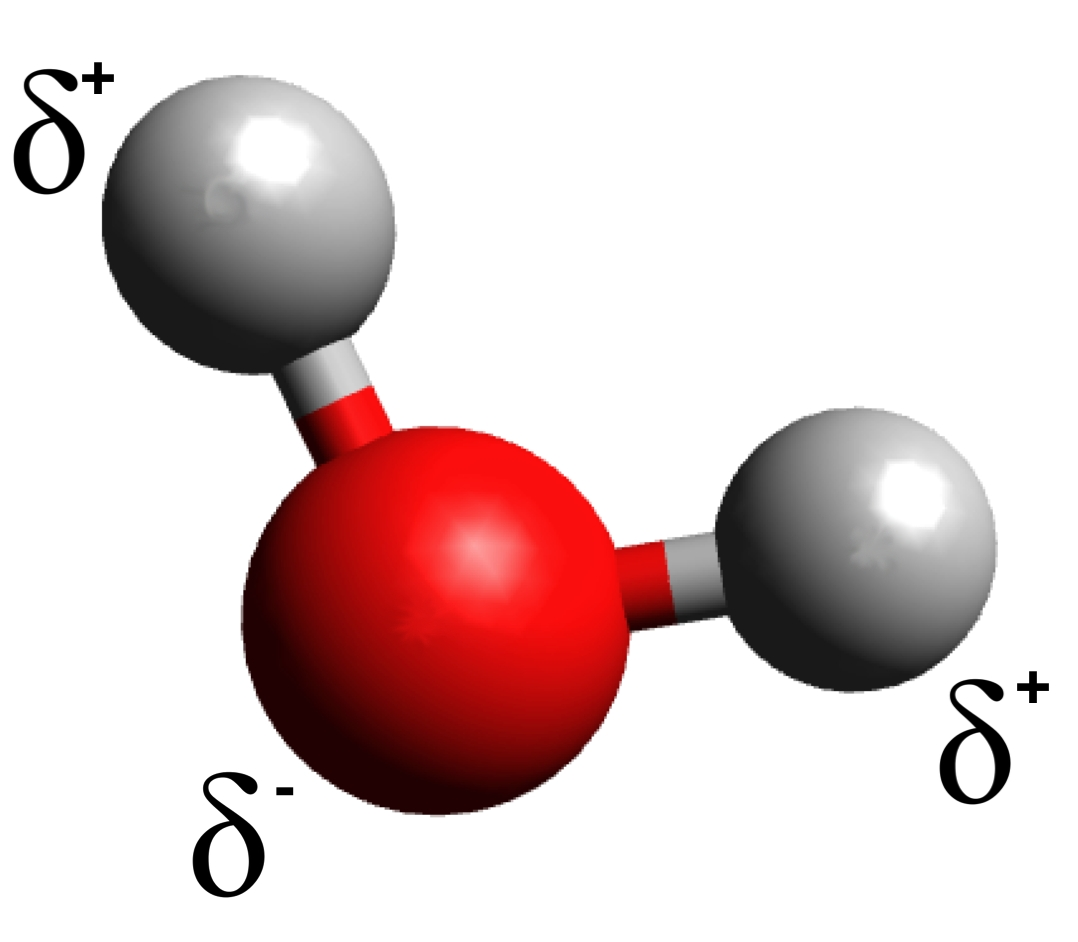
\includegraphics[width=.4\linewidth]{EnthalpyHydrogenBonds}
		\caption{Oxygen accepts electrons from Hydrogen}
	\end{subfigure}%
	\begin{subfigure}{.5\textwidth}
		\centering
		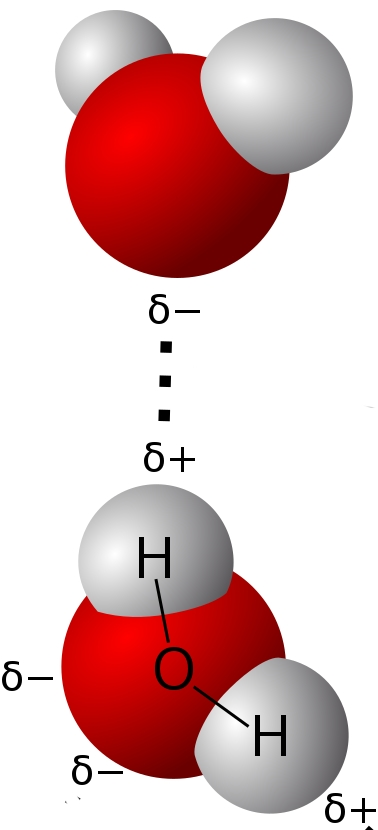
\includegraphics[width=.4\linewidth]{EnthalpyHydrogenBondMore}
		\caption{Positive ends bind to negative}
	\end{subfigure}
\end{figure}

\begin{figure}[H]
	\caption{The most important hydrogen bonds for biology} \label{fig:MajorHydrogenBonds} 
	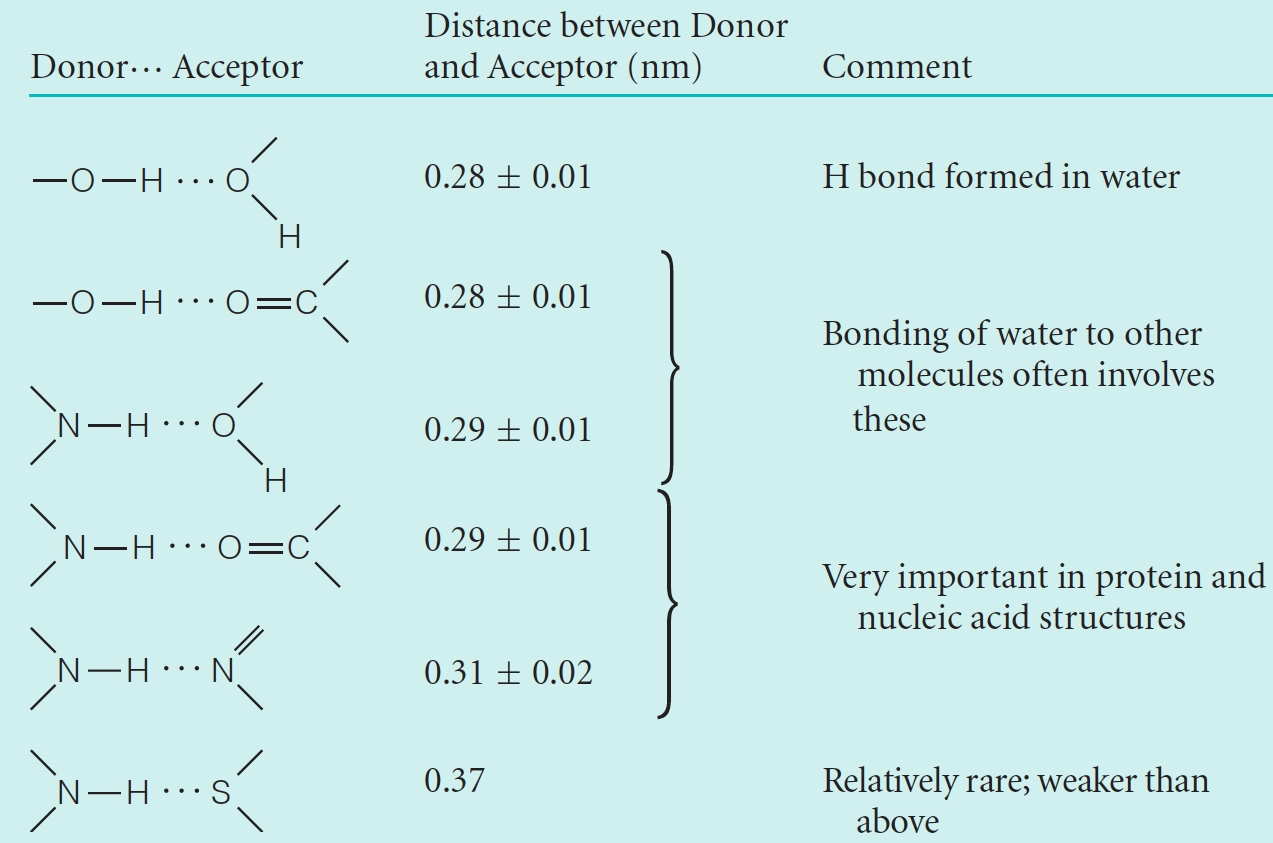
\includegraphics[width=0.9\textwidth]{MajorHydrogenBonds}
\end{figure}

Water has an entropic contribution: it can form many hydrogen bonds	with itself--Figure \ref{fig:Water_H_Bonds}--about 2 or 3 at a time. Molecules change conformation more frequently than once pers second.
\begin{figure}[H]
	\centering
	\caption{Water can form many hydrogen bonds	with itself} \label{fig:Water_H_Bonds} 
	\begin{subfigure}{.66\textwidth}
		\centering
		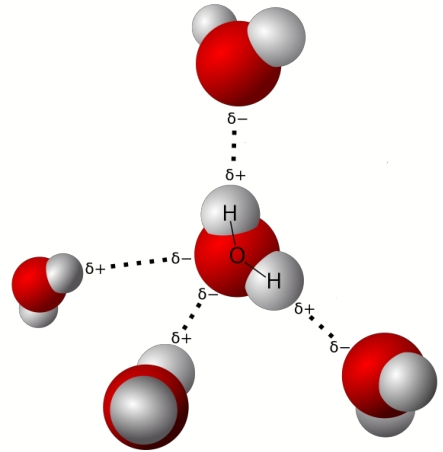
\includegraphics[width=.4\linewidth]{Water_H_Bonds}
		\caption{Water can bind to 2 or 3 others}
		\label{fig:sub1a}
	\end{subfigure}%
	\begin{subfigure}{.33\textwidth}
		\centering
		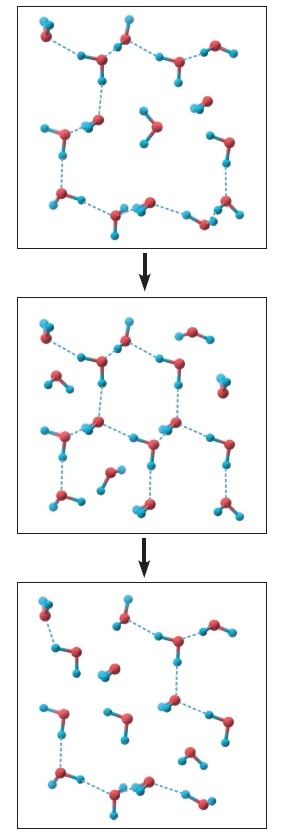
\includegraphics[width=.4\linewidth]{Water_H_Bonds_structure.jpg}
		\caption{Hydrogen bonds constantly change}
		\label{fig:sub2a}
	\end{subfigure}
\end{figure}

\begin{itemize}
	\item Water is good at interacting with polar or charged molecules
	\item ''Like dissolves like''
\end{itemize}

Water is good at interacting with polar or charged molecules. Figure \ref{fig:NonCovalentBonds} shows Sodium Chloride dissolved in water: the Sodium interacts with Oxygen, and Chloride with Hydrogen. This is a little stronger than a water-water interaction, so enthalpy is favoured over the entropic contribution.
\begin{figure}[H]
	\caption{Water is good at interacting with polar or charged
		molecules} \label{fig:NonCovalentBonds} 
	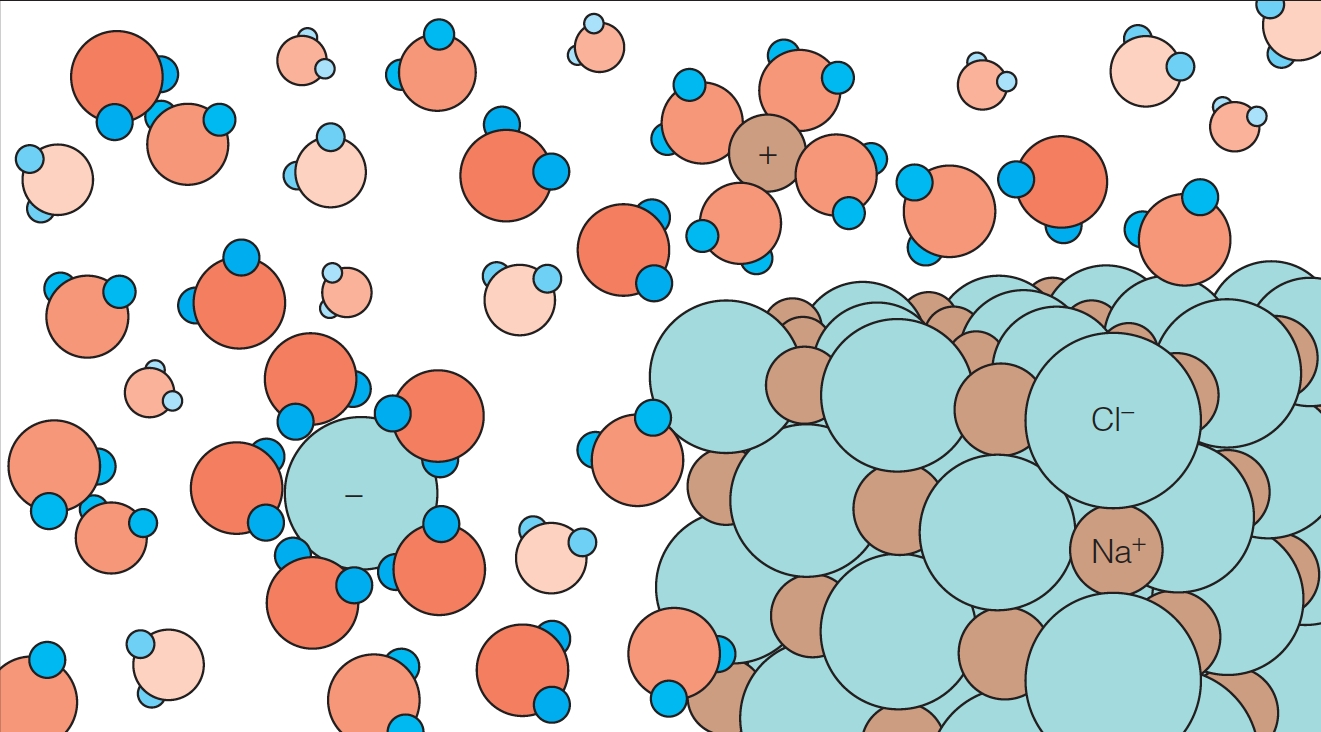
\includegraphics[width=0.9\textwidth]{NonCovalentBonds}
\end{figure}

Oil in Water
\begin{itemize}
	\item Figure \ref{fig:Hexane} depicts the formation of \gls{gls:clathrate} structures – water cannot form hydrogen bonds with oils.
	\item In Figure \ref {fig:clathrate}, Oxygen atoms are shown in red. Hydrogens are shown for one pentagon of oxygens. This is entropically unfavourable, and is known as the hydrophobic effect--Figure \ref{fig:HydrophobicEffect}.
	\item The ordered structure may extend considerably
	further into the surrounding water.
\end{itemize}
\begin{figure}[H]
	\centering
	\caption{Oil in water} \label{fig:Hexane} 
	\begin{subfigure}{.4\textwidth}
		\centering
		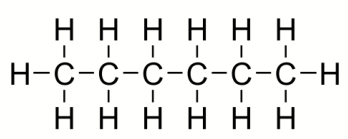
\includegraphics[width=.4\linewidth]{Hexane}
		\caption{Hexane is non-polar}
		\label{fig:hexane}
	\end{subfigure}%
	\begin{subfigure}{.6\textwidth}
		\centering
		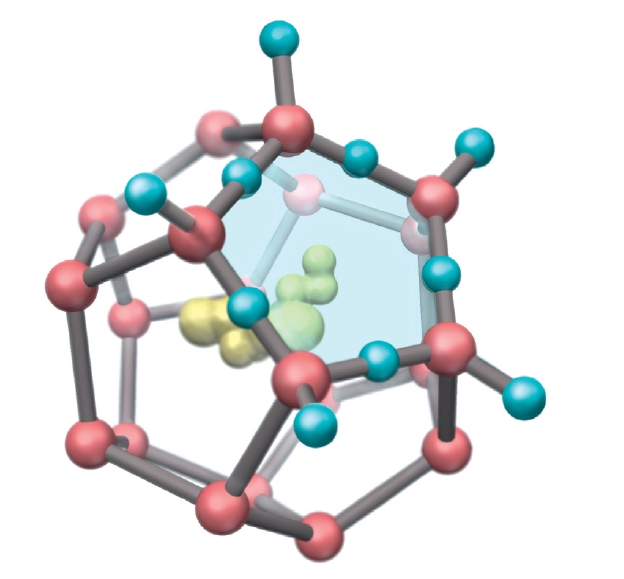
\includegraphics[width=.4\linewidth]{OilInWater.jpg}
		\caption{\Gls{gls:clathrate}: oxygen atoms are shown in red.}
		\label{fig:clathrate}
	\end{subfigure}
\end{figure}

Figure \ref{fig:HydrophobicEffect} depicts the hydrophobic effect: when oil interacts with water, it decreases entropy, which is thermodynamically unfavourable.
The hydrophobic effect leads to the formation of Lipid membranes-- Figure \ref{fig:LiquidMembraneFormation}. 
\begin{figure}[H]
	\caption{Hydrophobic effect} \label{fig:HydrophobicEffect} 
	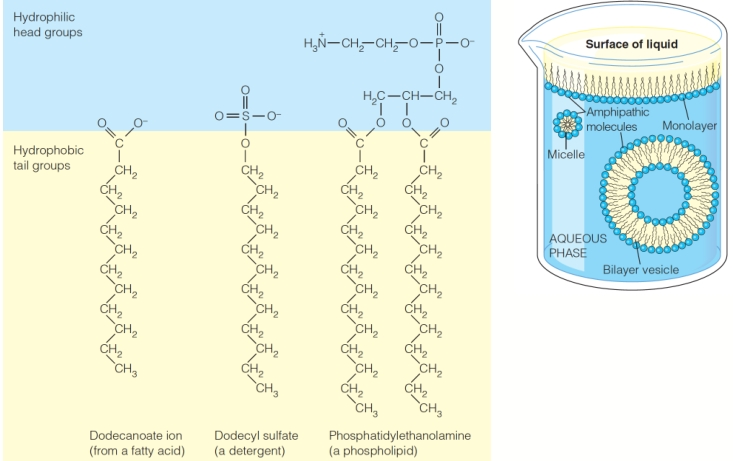
\includegraphics[width=0.9\textwidth]{HydrophobicEffect}
\end{figure}

Lipid membrane formation is depicted in Figure \ref{fig:LiquidMembraneFormation}.

\begin{itemize}
	\item Provides spatial organization within the cell
	\item Allows chemical gradients to generate energy
	\item Individuates populations to allow for Darwinian selection
\end{itemize}

\begin{figure}[H]
	\caption{Lipid membrane formation} \label{fig:LiquidMembraneFormation} 
	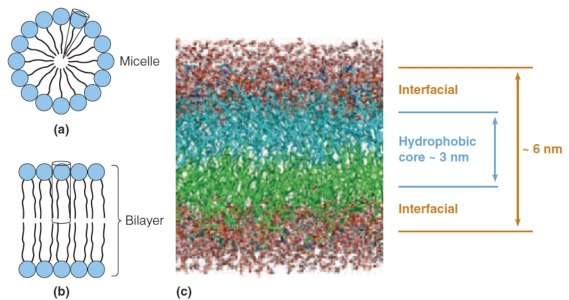
\includegraphics[width=0.9\textwidth]{LiquidMembraneFormation}
\end{figure}

Water also organizes material through Protein Folding, Figure \ref{fig:ProteinFolding} 
\begin{figure}[H]
	\caption{Protein folding} \label{fig:ProteinFolding} 
	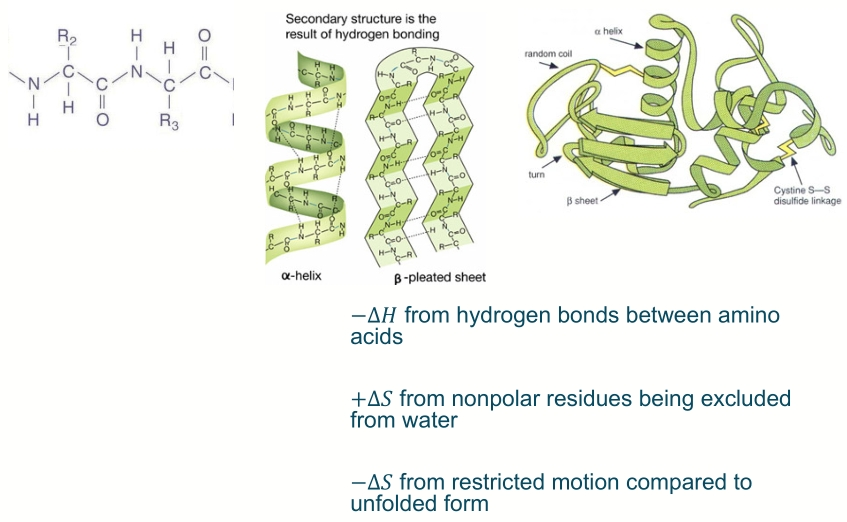
\includegraphics[width=0.9\textwidth]{ProteinFolding}
\end{figure}

 Relevance to origins of life?
\begin{itemize}
	\item Are proteins necessary in first life?
	\item Are membranes necessary in first life?
	\item Is water necessary for life?
\end{itemize}

Even in the RNA world, where RNA can fold and catalyze reaction, folding would be driven by entropy in part. Water is only solvent that has this high entropy. Ammonia can form hydrogen bonds, but they aren't as strong as water. Maybe water is the favoured solvent for life everywhere.

\cite{ball2017water}

\section{Kinetic vs. Thermodynamics – Assembly Constraints}

Lecturer: Chris Butch

\begin{itemize}
	\item \gls{gls:kinetics}  \glsdesc{gls:kinetics}
	\item \gls{gls:thermodynamics} \glsdesc{gls:thermodynamics}
\end{itemize}

Biomacromolecules are Kinetic Assemblies
\begin{itemize}
	\item Chemically: Amino Acids and Nucleic Acids are polymerized using energy from polyphosphates
	\item Structurally: Many nucleic acid structures, and most 	protein structures are kinetic minima, but not thermodynamic minima
	\begin{itemize}
		\item  Prion diseases involve an autocatalytic transition from the native kinetic state to a (more)stable thermodynamic state.
	\end{itemize}
\end{itemize}

Figure \ref{fig:prions} shows the PrP protein. Some energy is released by folding into the normal state, which is kinetically stable, but not thermodynamically stable--\cite{dee2016comparing}. Plaques are the lowest energy state. It is difficult to fight disease as this is uphill.

\begin{figure}[H]
	\caption{The PrP protein is stable kinetically , but not thermodynamically.} \label{fig:prions} 
	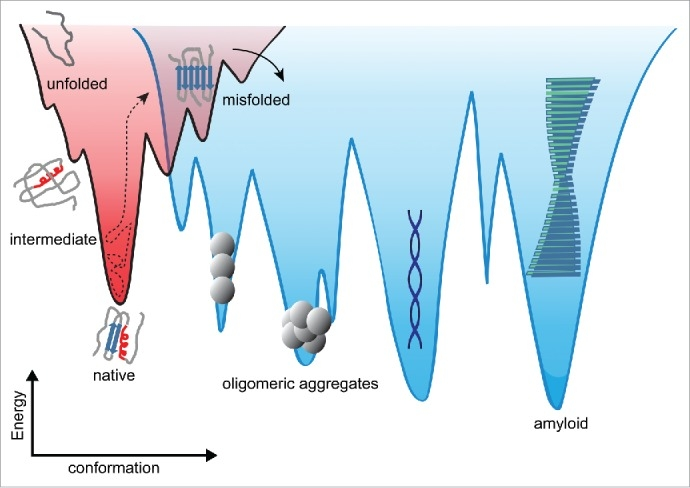
\includegraphics[width=0.9\textwidth]{prions}
\end{figure}

This is also a question for origins of life--Figure \ref {fig:EnergyForOrigin}--\cite{mast2013escalation}
\begin{figure}[H]
	\caption{How do we drive reaction to kinetic state?} \label{fig:EnergyForOrigin} 
	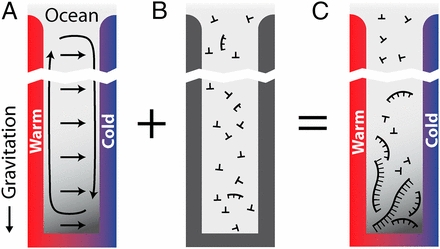
\includegraphics[width=0.9\textwidth]{EnergyForOrigin}
\end{figure}

\textbf{Open Questions}
\begin{itemize}
	\item Do environments exist where biological building
	blocks such as amino acids are
	thermodynamically favored, but exploration of
	their sequence space is kinetically favored?
	\item How do chemical systems utilize environmental
	energy to form kinetic assemblies?
\end{itemize}

See \cite{pross2017and},\cite{semenov2016autocatalytic},\cite{pross2008can}, \cite{pross2005emergence}.

\section{Chemical Configurations: Proteins and DNA}

Lecturer: Sarah Maurer

Figure \ref{fig:PrebioticMix} shows the chemicals observed in a Miller-Urey type experiment after \cite{podlech2001origin}. This list isn't what you'd expect to observe if you chopped up modern life.
\begin{figure}[H]
	\caption{Prebiotic Mixture from a Miller-Urey type experiment} \label{fig:PrebioticMix} 
	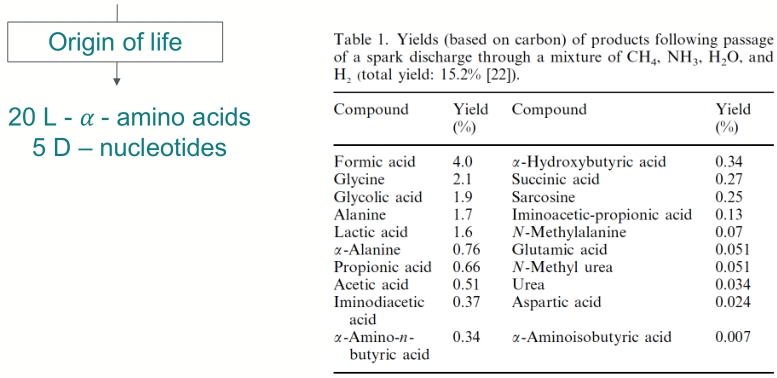
\includegraphics[width=0.9\textwidth]{PrebioticMix}
\end{figure}

\begin{itemize}
	\item How did life select from the list of Figure \ref{fig:PrebioticMix}? E.g. we don't use hydroxybuteric acid.
	\item Life uses L amino acids and D sugars \& nucleotides. How did this come about?
\end{itemize}

\begin{figure}[H]
	\caption{Chirality} \label{fig:Chirality1} 
	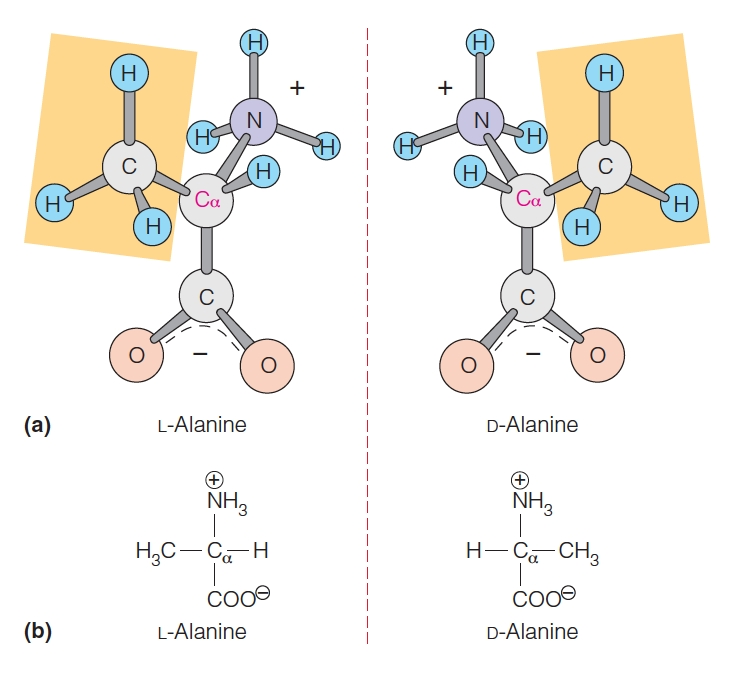
\includegraphics[width=0.9\textwidth]{Chirality1}
\end{figure}

How does chirality arise? Most chemical processes produce equal amounts. At one time it was thought that chirality was a marker for life, but we now know that meteorites are enriched for L--Figure \ref{fig:Chirality2}  \cite{pizzarello2012large}.
\begin{itemize}
	\item L-amino acids – enriched by meteorites--somehow?
	\item D - sugars (also in nucleotides)--enriched by L - amino acids.
	\item So it is enough if we can explain L-amino acids.
\end{itemize}
\begin{figure}[H]
	\caption{Meteorites are enriched for L} \label{fig:Chirality2} 
	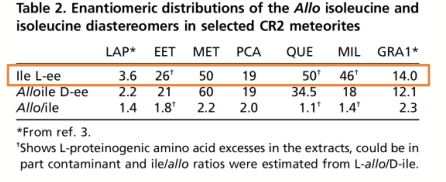
\includegraphics[width=0.9\textwidth]{Chirality2}
\end{figure}


Sarah has added (Forum):
\begin{quotation}
	I know I made it sound like the solution to the chirality of molecules has been found. However this is actually an active area of debate within the community. Many chemical strides have been made in the past 20 year towards make enantiomeric excesses abiotically, and therefore chirality is not specifically thought of as a biological phenomenon. However, to date, there has not been a robust mechanism of generating D-sugars and L-amino acids, although we certainly have seen hints to interstellar generation of excess.
	
	In this article \cite{soai2019role} symmetry breaking for a non-biological molecule can be induced by a variety of mechanisms including circularly polarized light and crystal structure.
	
	In this paper\cite{tassinari2019enantioseparation} The authors use a magnet to crystallize opposite enantiomers of amino acids!
	
	I often refer to chirality as ''the rabbit's hole'' (Alice in Wonderland reference) as we have many mechanisms to chase, but it is not obvious if they will get us any closer to understanding origins of life. Or perhaps it is the key to understanding it?
\end{quotation}
\newlength\mylength
\setlength\mylength{\dimexpr.33\columnwidth-2\tabcolsep-0.33\arrayrulewidth\relax}
\begin{tabular}{|p{\mylength}| p{\mylength}|p{\mylength}| } \hline
	Biological& Alternatives&Remarks\\ \hline
	Amino acid&	hydroxy acids, thio acids, amino sulfonic- or amino phosphinic acids&Peptide is a very strong bond compared to others. Also amine can hydrogen bond with carboxyl, which is useful for secondary structures. \\ \hline
	Residues at the $\alpha$ carbon& $\beta$-, $\gamma$-, or $\delta$-amino acids, or other derivatives&Maybe $\alpha$ more available; also products more stable\\ \hline
	20 exactly& More or less than 20&\\ \hline
	Our specific set of 20 &Other amino acids that were available prebiotically; e.g. why valine and not norvaline?&\\ \hline
\end{tabular}


Figure \ref{fig:PrebioticAminoAcids} \cite{cleaves2010origin} shows amino acids found in the Murchison meteorite and spark discharges. Why were black ones selected? Maybe they are more stable, or maybe they were incorporated, but later selected against.

\begin{figure}[H]
	\caption{Amino acids found in the Murchison meteorite and spark discharges} \label{fig:PrebioticAminoAcids} 
	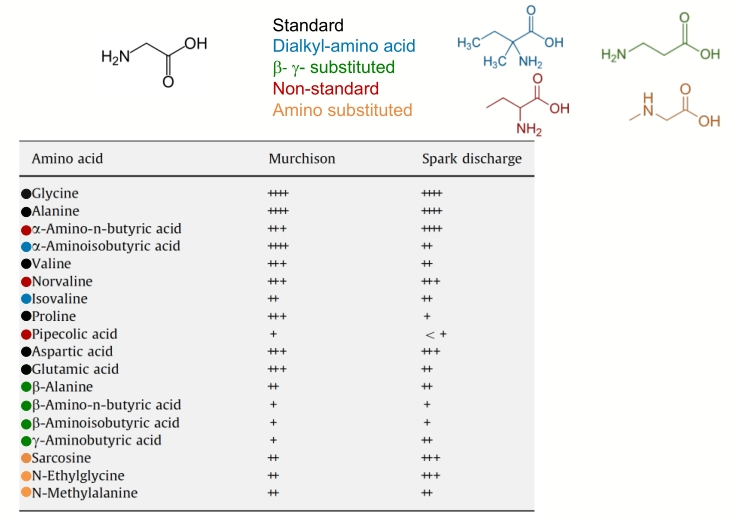
\includegraphics[width=0.9\textwidth]{PrebioticAminoAcids}
\end{figure}

Figure \ref{fig:ReducedAlphabet} attempts to reconstruct alphabet at origin; red asterisks are proteins that are not found in prebiotic experiments. The amino acids that have low abundances are the ones that are less likely to be formed. So maybe we started with just a few amino acids and later figured how to synthesize more, and this gave more functionality. 
\begin{figure}[H]
	\caption{Deconstructed Alphabet at time of origin of life} \label{fig:ReducedAlphabet} 
	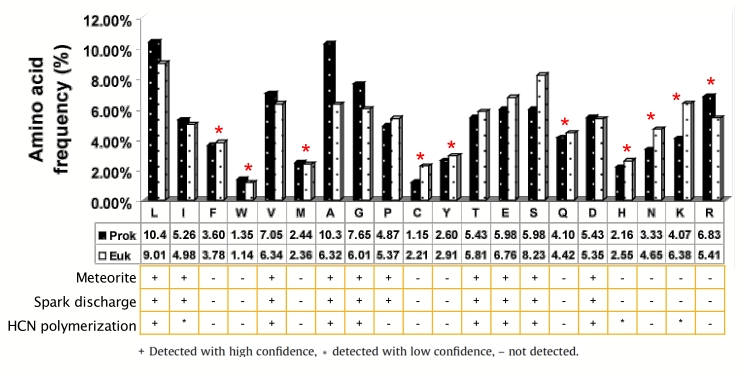
\includegraphics[width=0.9\textwidth]{ReducedAlphabet}
\end{figure}

\begin{figure}[H]
	\centering
	\caption{DNA/RNA much larger than proteins} \label{fig:NucleicAcidStructure} 
	\begin{subfigure}{.5\textwidth}
		\centering
		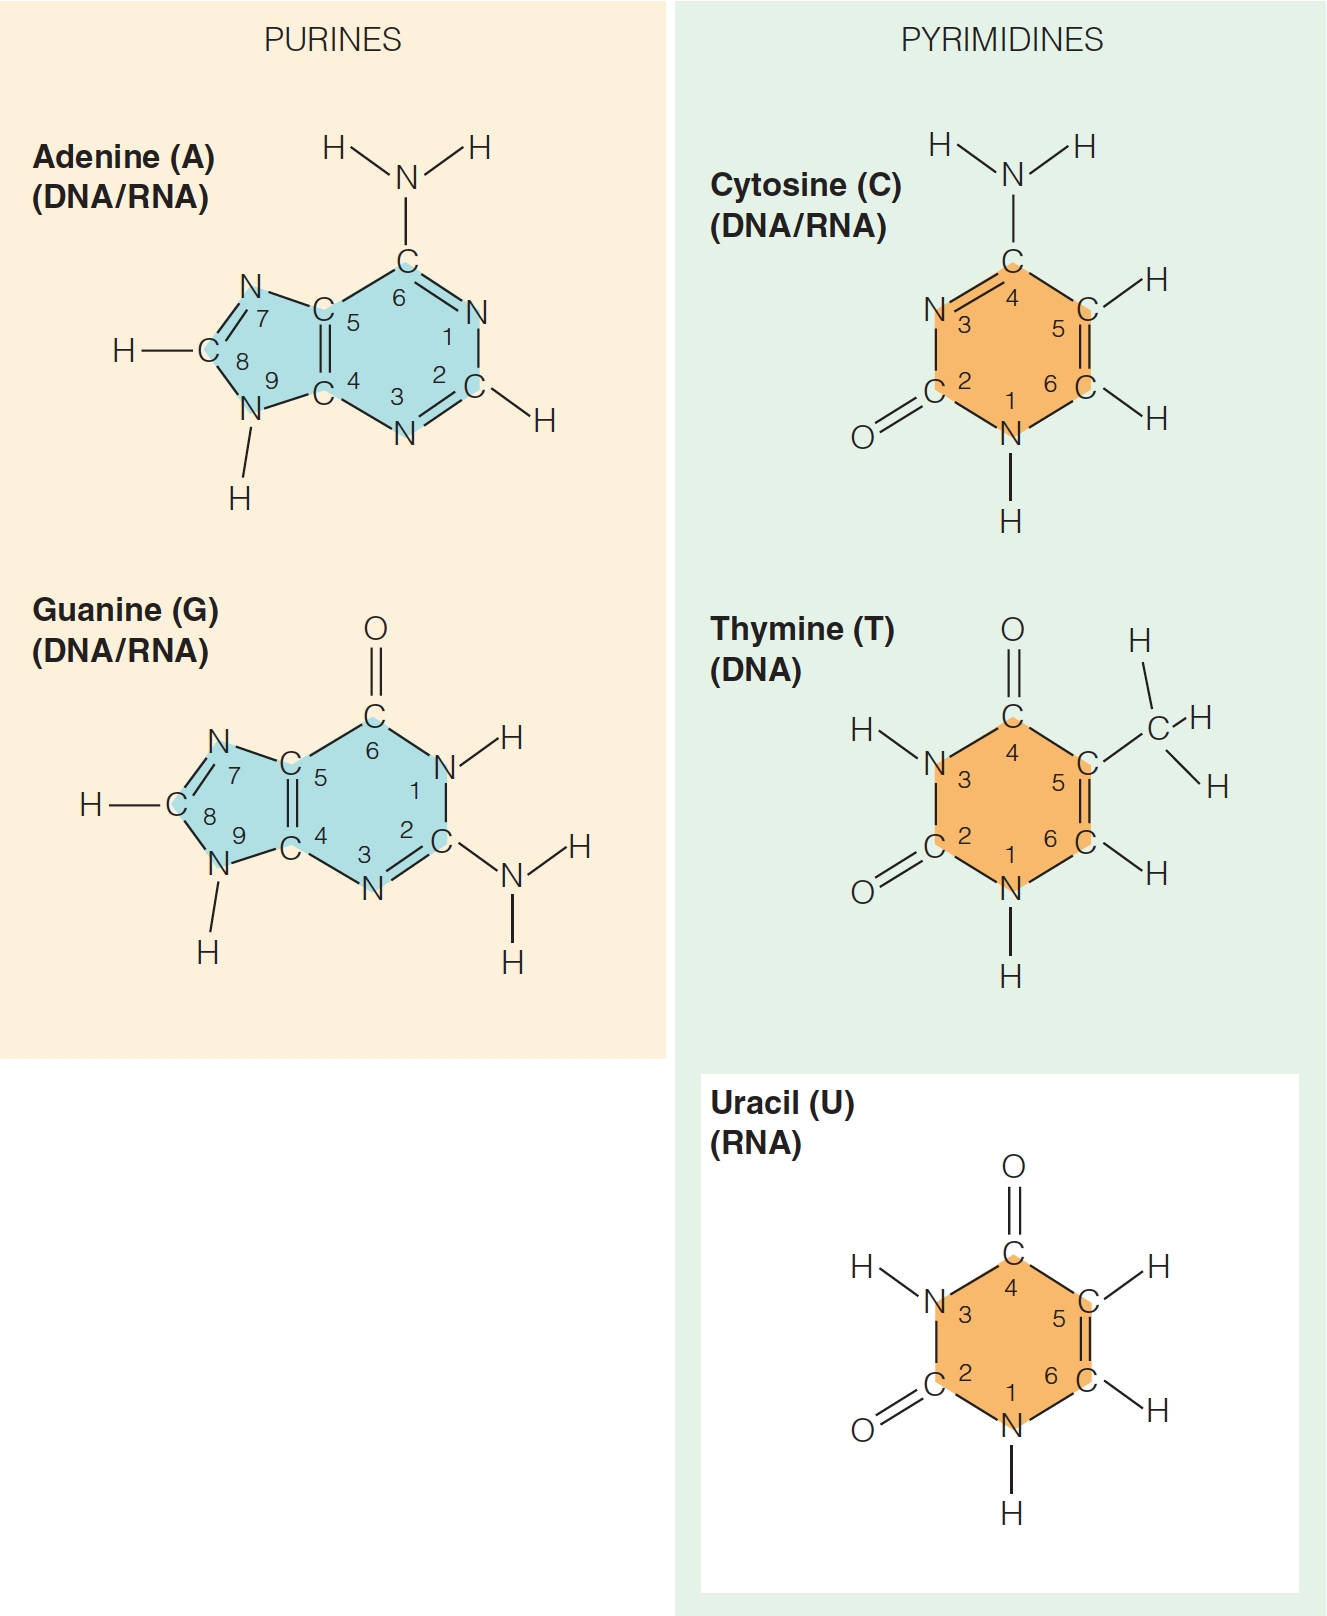
\includegraphics[width=.9\linewidth]{NucleicAcidStructure1}
	\end{subfigure}%
	\begin{subfigure}{.5\textwidth}
		\centering
		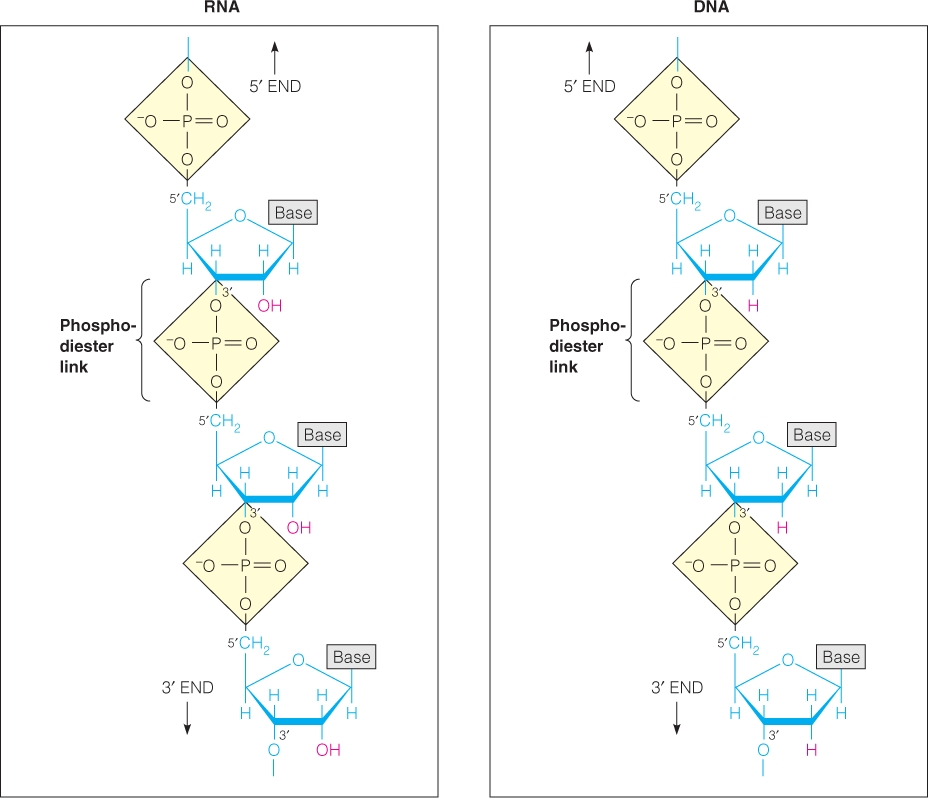
\includegraphics[width=.9\linewidth]{NucleicAcidStructure2}
	\end{subfigure}
\end{figure}

\begin{figure}[H]
	\caption{There are natural modified DNAs} \label{fig:NaturalxNA} 
	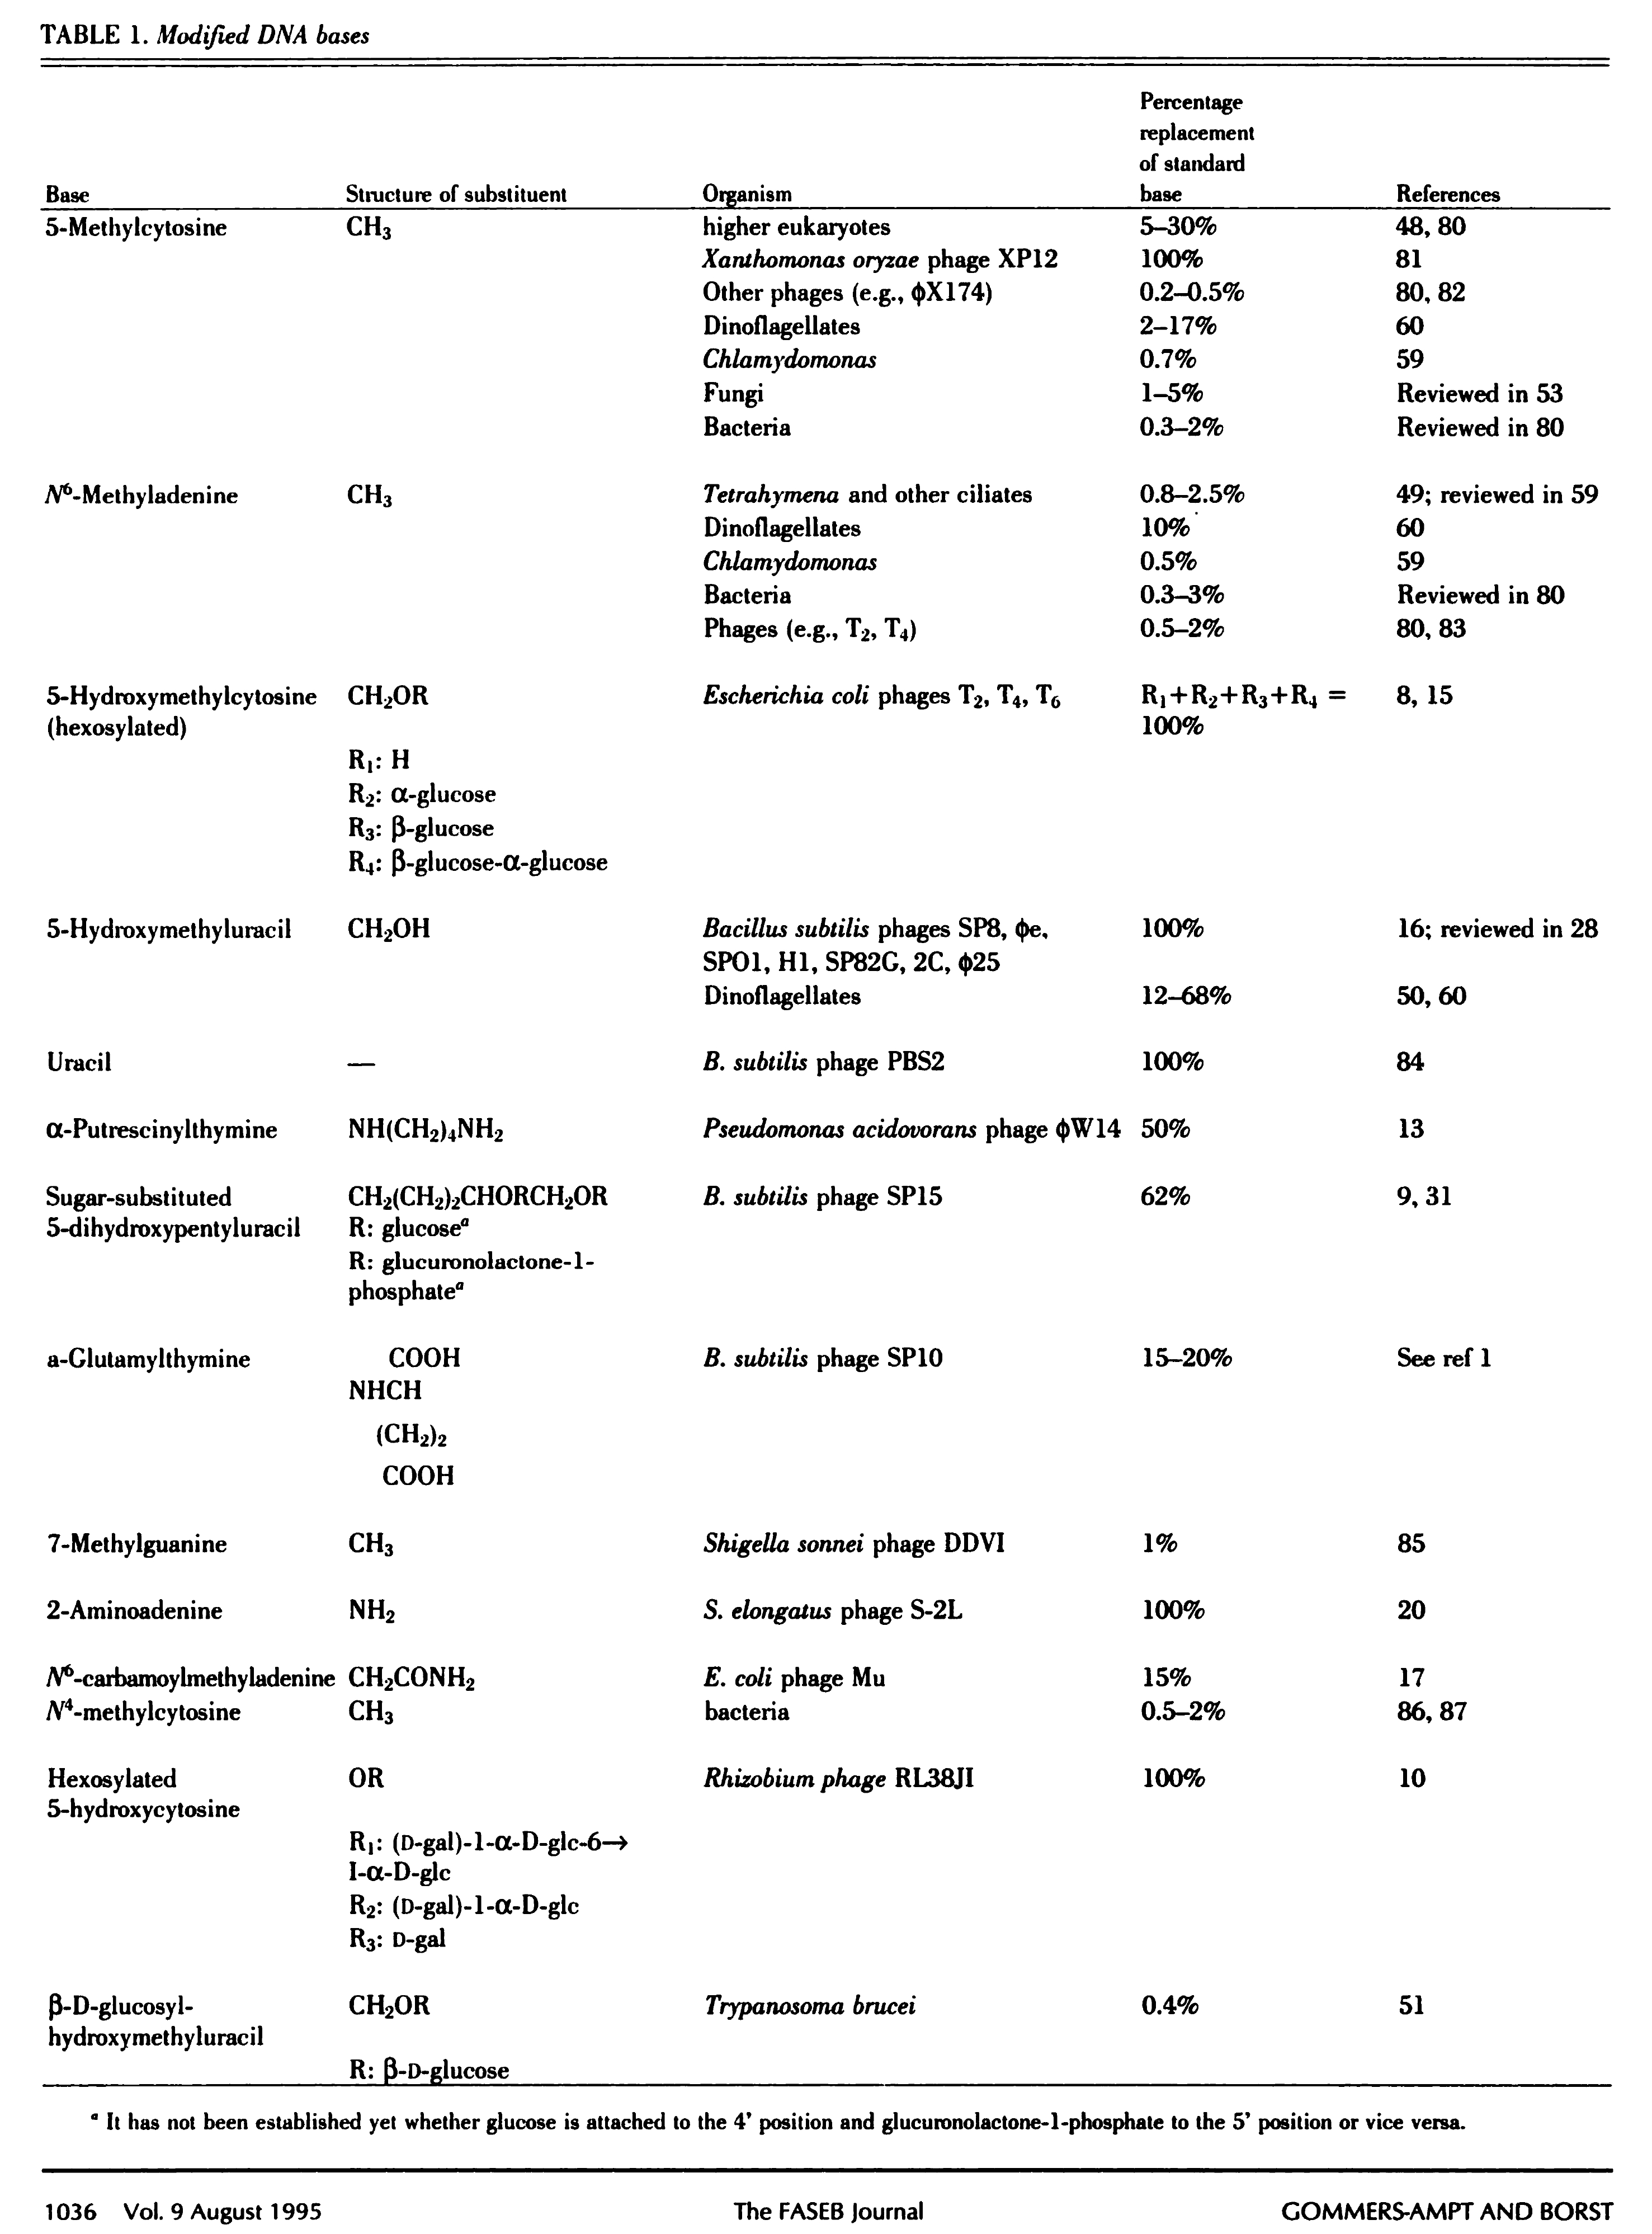
\includegraphics[width=0.9\textwidth]{NaturalxNA}
\end{figure}

Figure \ref{fig:WhyRibose} depicts the 4 forms of ribose\cite{wei2009permeation}.
\begin{itemize}
	\item Furanoses have $CH_2OH$, needed for polymerization
	\item Need a $beta$ to attach base
	\item Ribose is the only pentose that has plenty of $\beta$ furanose. 
\end{itemize}
\begin{figure}[H]
	\caption{Why Ribose?} \label{fig:WhyRibose} 
	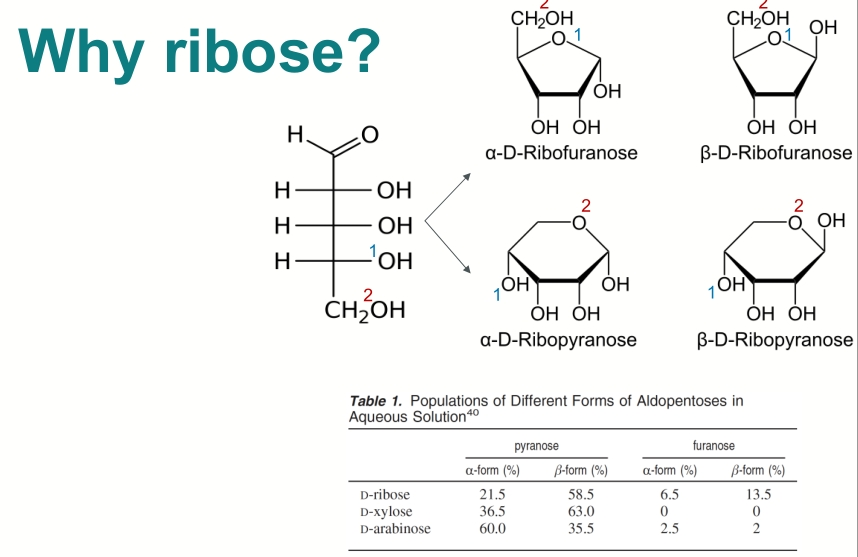
\includegraphics[width=0.9\textwidth]{WhyRibose}
\end{figure}

\begin{itemize}
	\item 5-carbon easier to synthesize than 6-, 7-, etc;
	\item shorted sugars don't form ring structure;
	\item so pentoses are cheapest sugar with ring structure.
\end{itemize}

Ribose has an almost unique permeability, so it can enter membrane, pick up phosphate, but cannot get out again! Maybe it was selected for speed?

\begin{figure}[H]
	\caption{These sugars have been tested and can replace Ribose} \label{fig:AlternativeSugars} 
	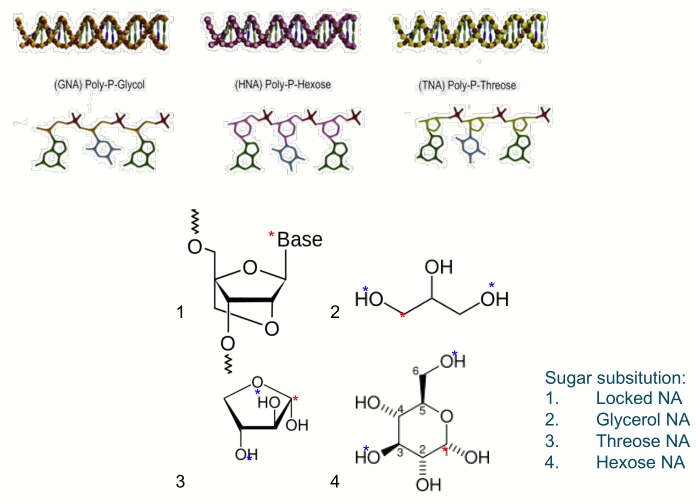
\includegraphics[width=0.9\textwidth]{AlternativeSugars}
\end{figure}

\begin{figure}[H]
	\caption{Can add a third type of base pair} \label{fig:ExpandGeneticCode} 
	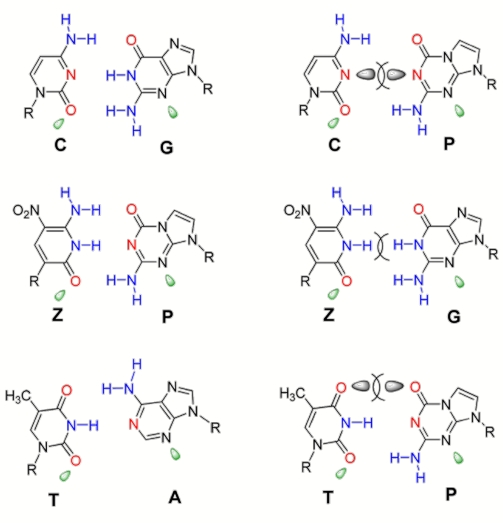
\includegraphics[width=0.9\textwidth]{ExpandGeneticCode}
\end{figure}

Can also modifiy phosphate, as shown in Figure \ref{fig:PhosphateModification}. Oxygen-substitution generates chirality
\begin{itemize}
	\item Boron
	\item Sulfur
	\item Selenium
	\item Hydrogen
\end{itemize}

Improves stability in vivo--useful for gene therapy.

\begin{figure}[H]
	\caption{Phosphate Modification} \label{fig:PhosphateModification} 
	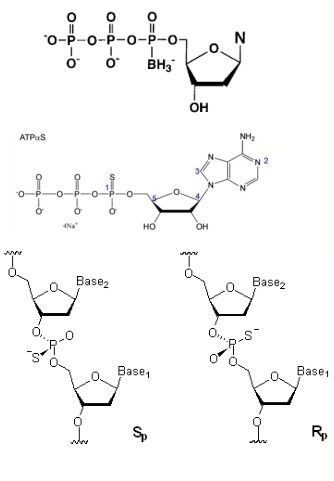
\includegraphics[width=0.9\textwidth]{PhosphateModification}
\end{figure}

Figure \ref{fig:PossibleModifications} shows there are many possible alternatives to DNA/RNA.
\begin{figure}[H]
	\caption{Possible Modifications to DNA} \label{fig:PossibleModifications} 
	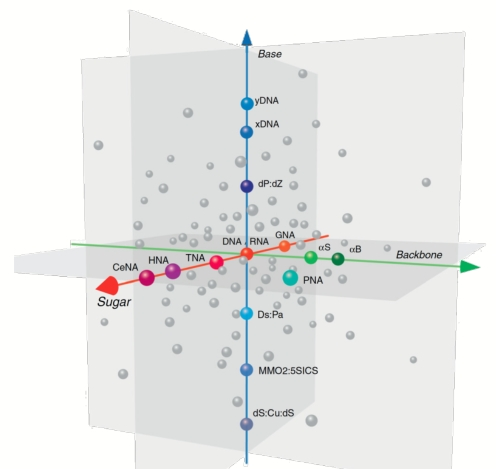
\includegraphics[width=0.9\textwidth]{PossibleModifications}
\end{figure}

 More complex amino acids were likely selected based on other criteria (not 
availability), possibly with later adaptation into biochemistry
\begin{itemize}
	\item  Sulfur containing
	\item Aromatics
	\item Nitrogen containing
\end{itemize}
Constraints on origin of amino acids:

\begin{itemize}
	\item  Prebiotic availability
	\item  Metabolic accessibility/compatibility
	\item  Evolutionary history/functional utility
\end{itemize}

How did life choose?

\begin{itemize}
	\item Prebiotic selection:
	\begin{itemize}
		\item 	Availability
		\item Stability of monomers
		\item Stability of polymers
	\end{itemize}
	Biotic selection:
	\begin{itemize}
		\item 	Cost of biosynthesis
		\item Increased functionality
	\end{itemize}
\end{itemize}
Would it choose these twice?

\section{Early Metabolisms}

\subsection{Introduction}

Lecturer: Kate Adamala

All life comes from a starting population of cells--\gls{gls:LUCA}. These cells were the ancestors of all subsequent life, their metabolism shared similarities. We know that the earliest metabolism shared certain features(Figure \ref {fig:LUCA_cell}):
\begin{itemize}
	\item Lipid synthesis--building membranes isolating cells from their surroundings;
	\item Energy: metabolism had to produce \gls{gls:ATP};
	\item LUCA had to produce proteins based on genetic code.
\end{itemize}
\begin{figure}[H]
	\caption{All life comes from a starting population of cells LUCA} \label{fig:LUCA_cell} 
	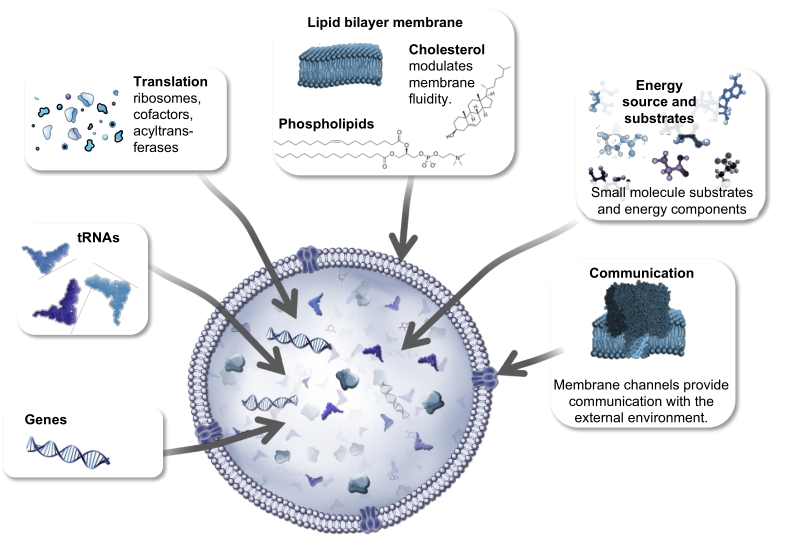
\includegraphics[width=0.9\textwidth]{LUCA_cell}
\end{figure}

Figure \ref{fig:LUCA_Environment} depicts a \textit{proposed} reconstruction of the metabolism of \gls{gls:LUCA}\cite{weiss2016physiology}. Since early Earth was anoxic, pathways do not use oxygen directly. The Figure is assumed to be near a hydrothermal vent.
\begin{figure}[H]
	\caption{Proposed main metabolic pathways of LUCA. } \label{fig:LUCA_Environment} 
	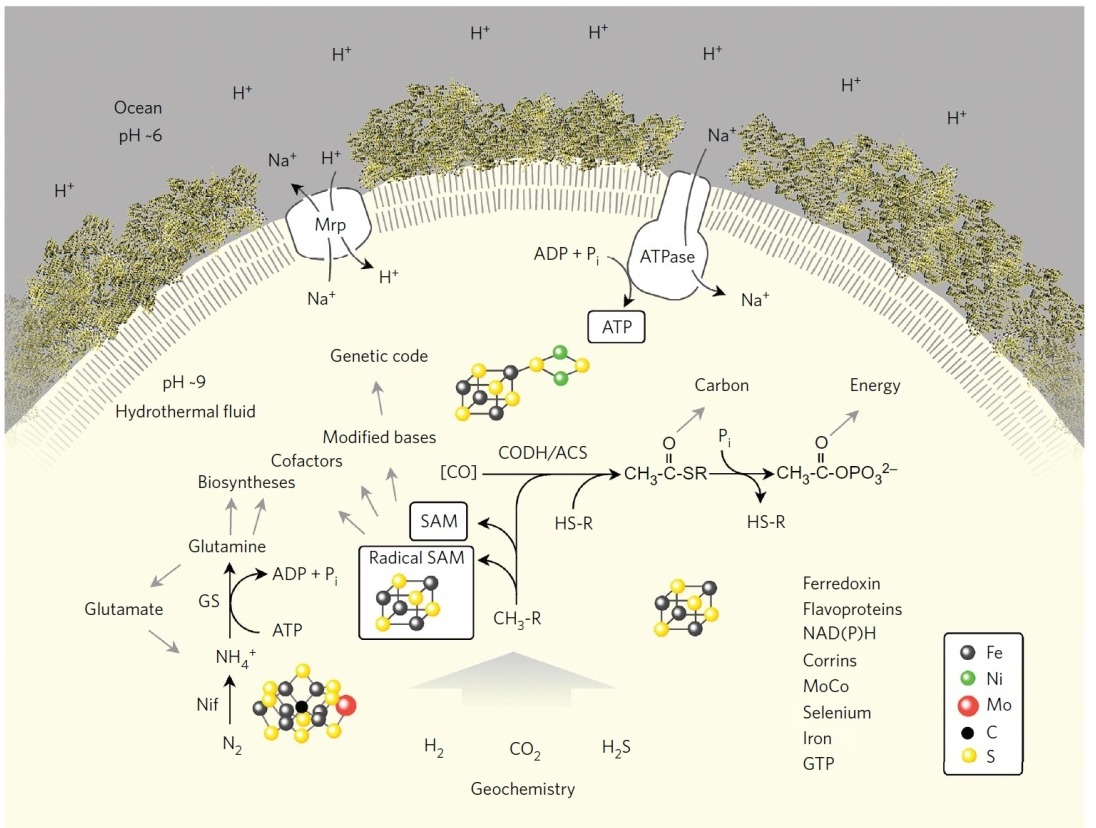
\includegraphics[width=0.9\textwidth]{LUCA_Environment}
\end{figure}

The process of taking inorganic carbon and converting it into origanic carbon building blocks is the key metabolic process of life--Figure \ref{fig:CarbonRules}. Carbon fixation must have been present in \gls{gls:LUCA}, but would have been simpler--fewer and less complex enzymes.
\begin{figure}[H]
	\caption{Carbon fixation} \label{fig:CarbonRules} 
	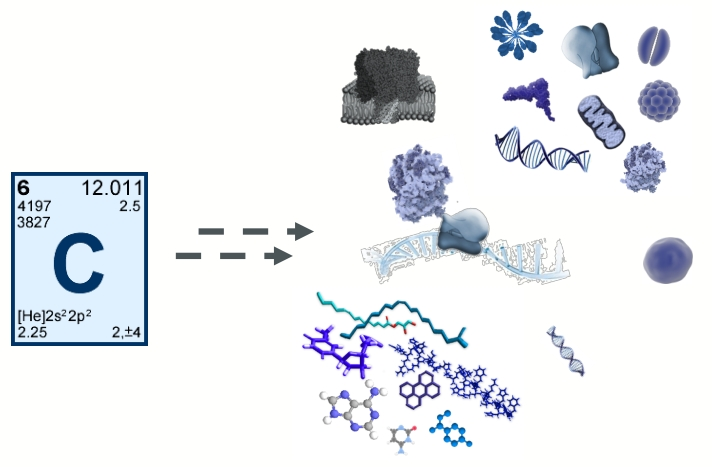
\includegraphics[width=0.9\textwidth]{CarbonRules}
\end{figure}

Synthesis of Membrane Lipids is another very important metabolic process. Modern cells have two families of Membrane Lipids--Figure \ref{fig:SynthsisMembraneLipids}--the difference is in how a glycerol molecule is attached. Synthesis of Membrane Lipids was still evolving at the time of LUCA. \cite{glansdorff2008last}.
\begin{figure}[H]
	\caption{Modern cells have two families of Membrane Lipids} \label{fig:SynthsisMembraneLipids} 
	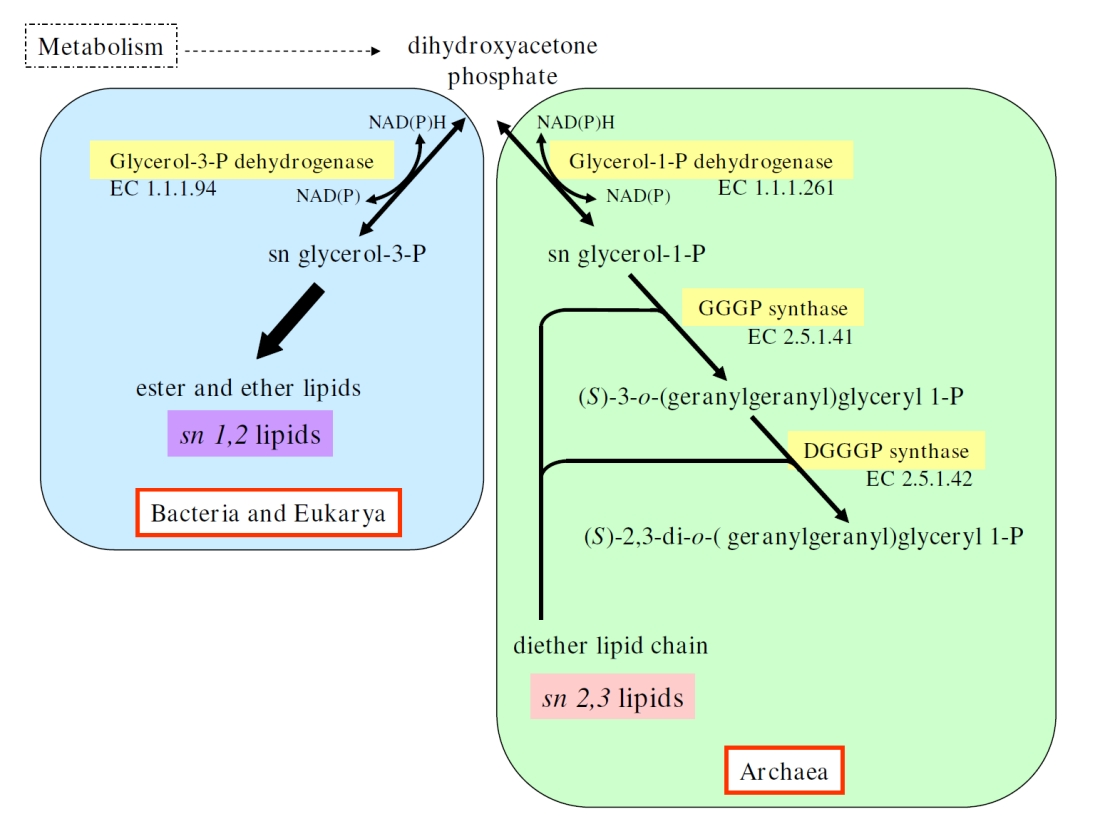
\includegraphics[width=0.9\textwidth]{SynthsisMembraneLipids}
\end{figure}

We can use this Lipid Synthesis Metabolism Comparison--\ref {fig:LipidSynthesisComparison}--as an example of evolution from earliest ancestors \cite{lombard2012early}. For some steps there is phylogenetic evidence that homologous mechanisms carried out a particular step or that the enzymes cannot be excluded. Differences between the modern domains of life have to have evolved from the simpler pathways of \gls{gls:LUCA}.
\begin{figure}[H]
	\caption{Lipid Synthesis Metabolism Comparison} \label{fig:LipidSynthesisComparison} 
	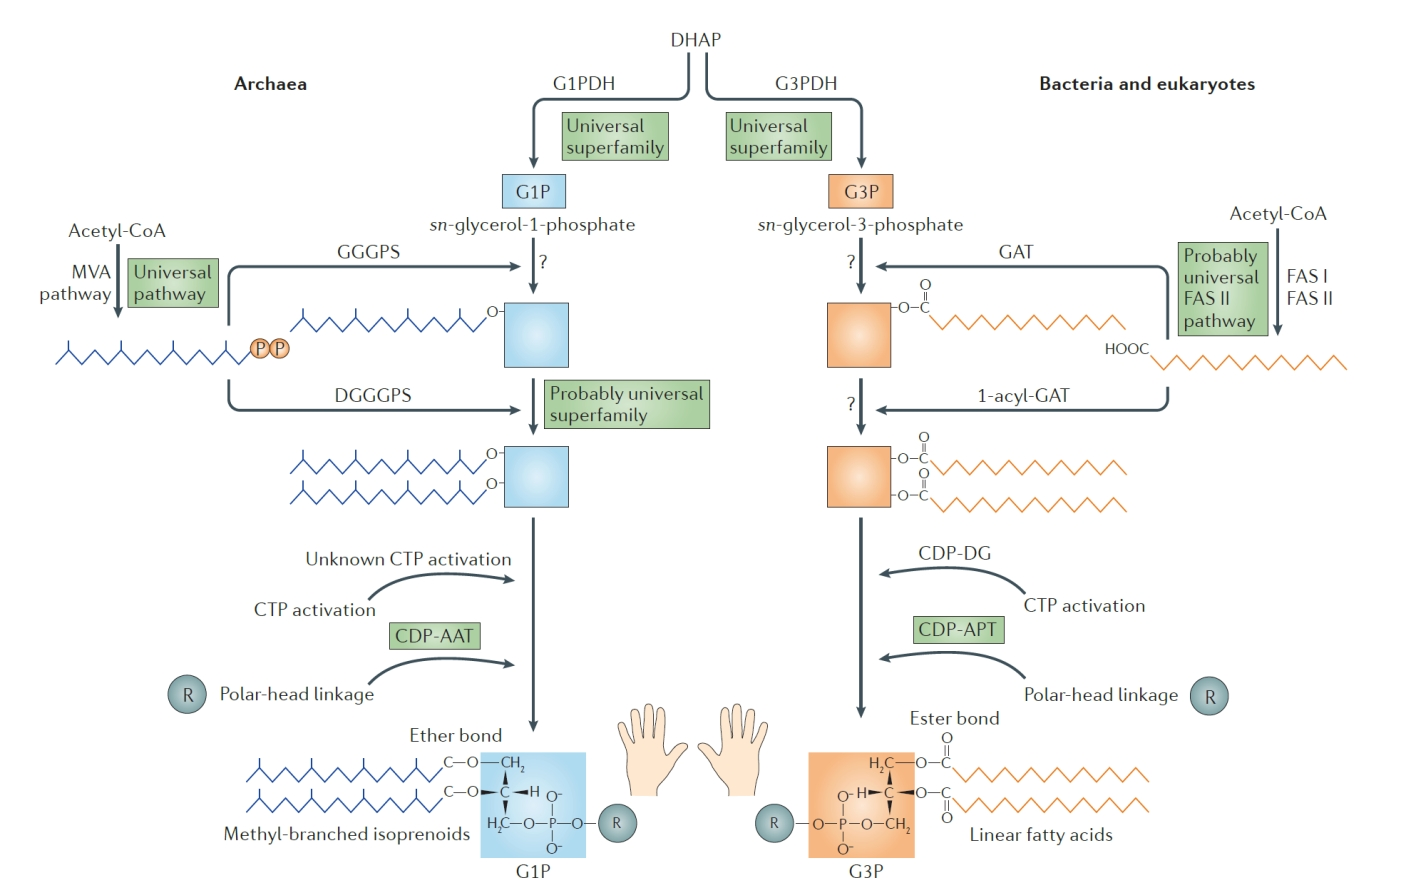
\includegraphics[width=0.9\textwidth]{LipidSynthesisComparison}
\end{figure}

See also \cite{bar2011survey}, \cite{fuchs2011alternative}.

\subsection{Energetics}

Lecturer: Sarah Maurer

We look at early metabolisms, and how they evolved into those we see today. 
Figure \ref{fig:ClassificationEnergyGeneration} shows various mechanisms for generating organisms. Chemoautotrophs convert $CO_2$ to reduced carbon; this lecture at the evolution of chemoautotrophy. We need to discuss redox reactions, as chemoautotrophs need to move electrons around.

\begin{figure}[H]
	\caption{Classification of energy generation in organisms} \label{fig:ClassificationEnergyGeneration} 
	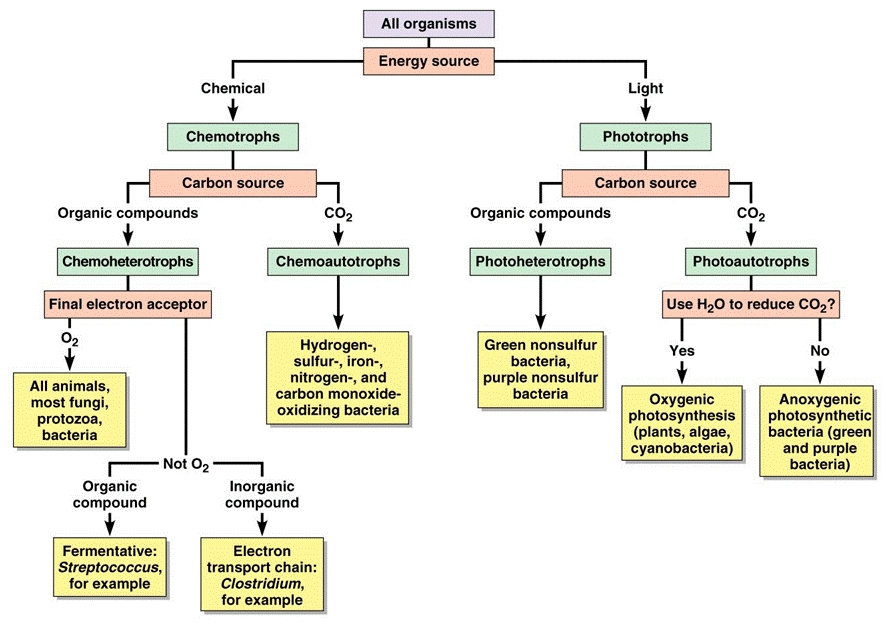
\includegraphics[width=0.9\textwidth]{ClassificationEnergyGeneration}
\end{figure}

We'll think of primordial respiration as a process of electron transfer from sources, such as $Fe^{2+}$ to acceptors--Figure \ref{fig:EvolutionMetabolism}\footnote{In Figure \ref{fig:EvolutionMetabolism}, \textit{retinal} should read \textit{retinol}.}. Free Oxygen would not have been available. Primordial respiration serves as the bases for all later respirations, e.g. the branch for chlorophyll. Later organisms evolve a way of using oxygen as it becomes free.
\begin{figure}[H]
	\caption{Evolution of Metabolism} \label{fig:EvolutionMetabolism} 
	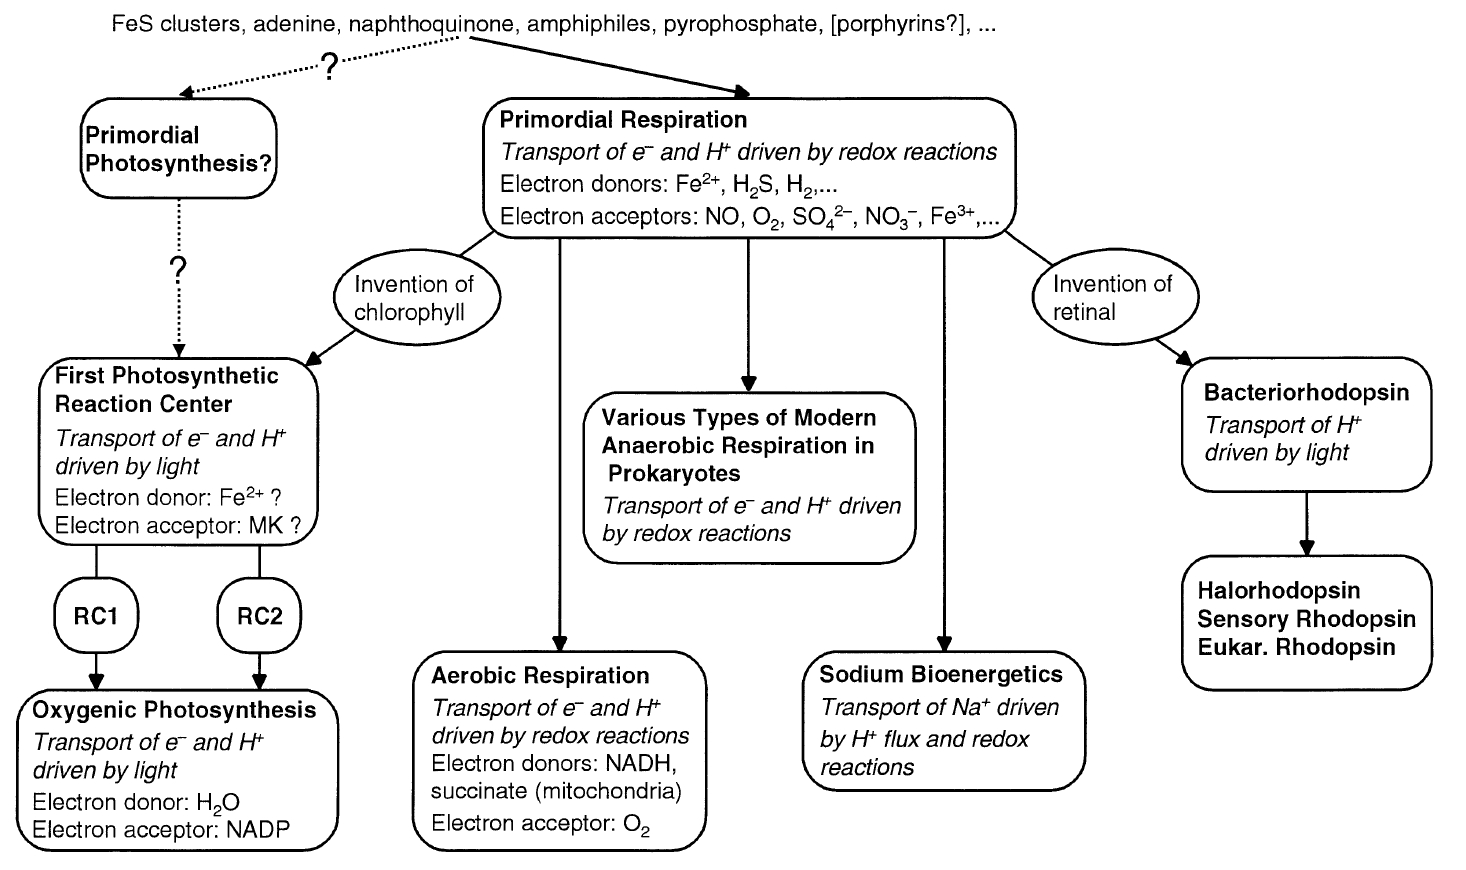
\includegraphics[width=0.9\textwidth]{EvolutionMetabolism}
\end{figure}

What would the first form of chemoautotrophy have looked like? Figure \ref{fig:Methanogenesis} \cite{costa2014metabolic} shows the reduction of carbon in $CO_2$ to $CH_4$. Figure \ref{fig:320px-Methanogenesis_cycle} \cite{wiki:methanogenesis} shows that this is accomplished by attaching $CO_2$ to a larger molecule, and then adding electrons until carbon arrives at its mot reduced form. 

\begin{figure}[H]
	\caption{Methanogenesis: $CO_2$ acquires electrons--in red} \label{fig:Methanogenesis} 
	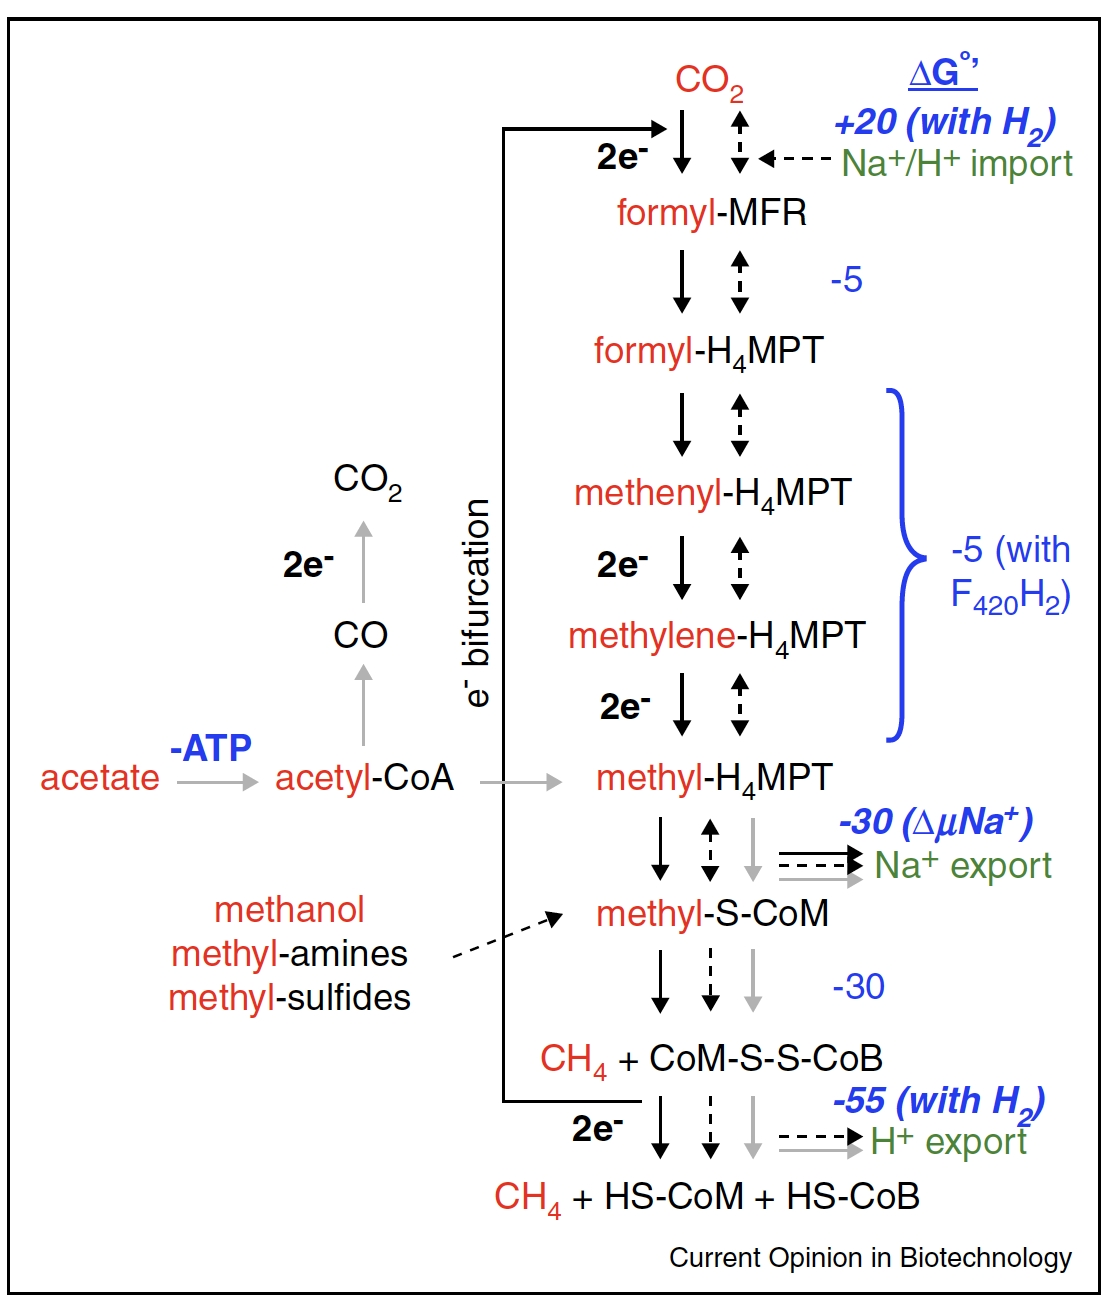
\includegraphics[width=0.9\textwidth]{Methanogenesis}
\end{figure}

\begin{figure}[H]
	\caption{Details of reduction of Carbon} \label{fig:320px-Methanogenesis_cycle} 
	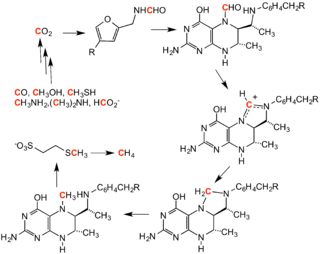
\includegraphics[width=0.9\textwidth]{320px-Methanogenesis_cycle}
\end{figure}

How might the earliest carbon fixation have looked? Figure \ref{fig:CarbonFixationMinerals} \cite{varma2018native} depicts one mechanism for fixing carbon on a mineral surface. Note the presence of pyruvate, which we use to generate ATP. If there is a simple, mineral bound, mechanism for methanogenisis, we think we have a good chance of recreating the actual primordial metabolism for chemoautotrophy in our labs today.
  
\begin{figure}[H]
	\caption{Carbon Fixation on Minerals (upper path)} \label{fig:CarbonFixationMinerals} 
	\includegraphics[width=0.9\textwidth]{CarbonFixationMinerals}
\end{figure}

How do electrons move when we have reduced carbon? Figure \ref{fig:ModernRedox} shows how this works today: a citric acid cycle, which generates FADH and $FADH_2$; we have fatty acid oxidation and glycolysis, protein degradation, etc. This all feeds electrons into our electron transport chain, which generates a proton gradient, eventually producing ATP. So essentially we want to take electrons and make a proton gradient that can be used later to drive ATP synthesis.

\begin{figure}[H]
	\caption{Modern Redox Chemistry: the Citric Acid Cycle} \label{fig:ModernRedox} 
	\includegraphics[width=0.9\textwidth]{ModernRedox}
\end{figure}

So what might our early redox chemistries have looked like? Figure \ref{fig:PrimordialRedox} \cite{sojo2016origin} depicts one proposal. At a hydrothermal group we could have a very fine layer of minerals that could act as a porous membrane or electron transfer membrane between alkaline hydrothermal vent and an acidic ocean. So there is already a proton gradient with a pH of 6. Electrons are transferred to $FeS$ and then onto $CO^2$. 

\begin{figure}[H]
	\caption{Primordial Redox Chemistry?} \label{fig:PrimordialRedox} 
	\includegraphics[width=0.9\textwidth]{PrimordialRedox}
\end{figure}

Other mechanisms have been proposed:
\begin{align*}
H_2 \rightarrow & 2H^+ + 2 e^- \text{, then electrons pushed to $CO^2$ to make formaldehyde}\\
FeS + H_2 S \rightarrow &Fe S_2 +H2\\
4H_2 +CO2 \rightarrow & CH_4 + 2H_2 O\\
4H_2 + 2HCO^-_3 + sH^+\rightarrow & CH_3OO^- + 2H_2O\\
H_2 + Fd_{ox} \rightarrow & Fd^{2-}_{red} + 2H^+ 
\end{align*}

\begin{figure}[H]
	\caption{Evolution of Redox Reactions} \label{fig:PrimordialRedox2} 
	\includegraphics[width=0.9\textwidth]{PrimordialRedox2}
\end{figure}

\section{Energy Harvesting}

Lecturer: Shawn McGlynn

\begin{itemize}
	\item Chemical reactions occur when concentrations change to accommodate energy differences between molecules.
	
	\item Equilibrium occurs at some mixture of A and B when energy is equalized. The final concentrations are achieved at equilibrium.
	
	\item At constant temperature and 	pressure, we refer 	to the energy that is available to do work as \textit{Gibbs Energy}, after J. Willard Gibbs.
	
	\item $\Delta G$ is the change in energy as a reaction tends towards equilibrium.
	
	\item Biology chains reactions, so one reaction that is energetically unfavourable ( $\Delta G > 0$) may become favourable if coupled to another with  $\Delta G < 0$. 
\end{itemize}


\begin{figure}[H]
	\caption{The cellular membrane 	can separate charge} \label{fig:EnergyHarvesting1} 
	\includegraphics[width=0.9\textwidth]{EnergyHarvesting1}
\end{figure}


\cite{simon2008organisation}

\section{Systematics and Limits of Metabolic Rates}

Lectrure: Chris Kempes


All present day life is encapsulated: bacteria are simple cells; eukaryotes have organelles, within cells, within multicellular organisms.
\begin{itemize}
	\item Which aspects of extant life are general and 	which are arbitrary?
	\item What can be said about encapsulation in general?
\end{itemize}

How do nutrients cross cell boundary to drive metabolism--Figure \ref{fig:Encapsulation1}?
\begin{figure}[H]
	\caption{Metabolism in Cells} \label{fig:Encapsulation1} 
	\includegraphics[width=0.9\textwidth]{Encapsulation1}
\end{figure}

We model this by the diffusion equation:
\begin{align*}
\frac{\partial C}{\partial t} =& \frac{D}{r^2} \frac{\partial}{\partial r}\big(r^2 \frac{\partial C}{\partial R} \big) \\
\frac{\partial C}{\partial t} =& 0 \text{, in the steady state.}\\
 \frac{D}{r^2} \frac{\partial}{\partial r}\big(r^2 \frac{\partial C}{\partial R} \big) =& 0 \text{, in the steady state.}\\
 r^2 \frac{\partial C}{\partial R} =& A {, say}\\
 C =& B - \frac{A}{r}\\
 \text{assume}& \\
 C =& C_{\infty}\text{, when $r=\infty$, then}\\
 C =& C_{\infty} - \frac{A}{r}
 \text{Further, assume}&\\
 C =& 0\text{, when $r=a$, then we have}\\
 C =& c_{\infty}\big(1 - \frac{a}{r}\big) 
\end{align*}

\begin{align*}
J \triangleq& -D \frac{\partial C}{\partial R}\text{, definition of Flux}\\
=& D C_\infty \frac{a}{r^2}\\
4 \pi a^2 J =& 4 \pi D a C_{\infty} \text{, total flux}
\end{align*}

This gives a limit on the reaction rate of reactions within cells, and shows it dependence on the cell size. 
% end of text 

% glossary
\printglossaries

% bibliography goes here
 
\bibliographystyle{unsrt}
\addcontentsline{toc}{section}{Bibliography}
\bibliography{origins}

\end{document}
